\documentclass{article}

%definitions for Formelsammlung

\usepackage[left=1.5cm,right=1.5cm,top=2.5cm,bottom=2cm,landscape]{geometry} 
\usepackage{multicol}
\usepackage[ngerman]{babel}
\usepackage{tabularx}
\usepackage{mathpazo}
\usepackage{mathtools}
\usepackage{amsmath}  
\usepackage{setspace} 
\usepackage{commath}
\usepackage[utf8]{inputenc}
%\usepackage[ansinew]{inputenc}  
\usepackage[T1]{fontenc}
\usepackage{lmodern} 
\usepackage{hyperref}
\usepackage{bigints}
\usepackage{array}
\usepackage{xcolor}
\usepackage{layouts}
\usepackage{siunitx}
\usepackage{wrapfig}
\usepackage{multirow,bigstrut}
\usepackage{trfsigns}
\usepackage{amssymb}
\usepackage{fancyhdr}
\usepackage{datetime}
\usepackage{pgfplots}
\usepgfplotslibrary{fillbetween}
\usepackage{listings}
\usepackage{steinmetz}
\usepackage{textcomp}
\usepackage[export]{adjustbox}
\usepackage{booktabs}

\setlayoutscale{0.5}

\DeclareMathOperator\arctanh{arctanh}
\DeclareMathOperator\arsinh{arsinh} 
\DeclareMathOperator\arcosh{arcosh}
\DeclareMathOperator\artanh{artanh}
\DeclareMathOperator\arcoth{arcoth} 
\DeclareMathOperator\sinc{sinc} 
\DeclareMathOperator\Real{Re} 
\DeclareMathOperator\Imag{Im} 
\DeclareMathOperator\sgn{sgn} 
\DeclareMathOperator\LPF{LPF} 
\DeclareMathOperator\Q{Q} 
\DeclareMathOperator\erf{erf} 


%colorCodes
\definecolor{listinggray}{gray}{0.9}
\definecolor{lbcolor}{rgb}{0.95,0.95,0.95}
\definecolor{lightGray}{gray}{0.1}

\definecolor{cOrange}{HTML}{996633}
\definecolor{cBlue}{HTML}{336699}
\definecolor{cGreen}{HTML}{339966}
\definecolor{cRed}{HTML}{993333}
\definecolor{cGray}{gray}{0.4} 



\setlength{\parindent}{0pt}
%\DeclareMathOperator\arctanh{arccot}
\newcolumntype{L}[1]{>{\raggedright\let\newline\\\arraybackslash\hspace{0pt}}m{#1}}
\newcolumntype{C}[1]{>{\centering\let\newline\\\arraybackslash\hspace{0pt}}m{#1}}
\newcolumntype{R}[1]{>{\raggedleft\let\newline\\\arraybackslash\hspace{0pt}}m{#1}}
\newcolumntype{Y}{>{\centering\arraybackslash}X}
\newcolumntype{Z}{>{\raggedleft\arraybackslash}X}
\newcommand{\fmm}{\displaystyle} 
\newcommand{\cn}[1]{\underline{#1}} 
\newcommand{\hlaplace}{\quad\laplace\quad}
\newcommand{\hLaplace}{\quad\Laplace\quad}
\newcommand{\rads}{\left[\frac{rad}{s}\right]}
\newcommand{\pol}{\textbf{\color{cRed}\texttimes}}
\newcommand{\nullstelle}{$\color{cBlue}\mathbf{\circ}$}
\newcommand{\symtrue}{\checkmark}
\newcommand{\symfalse}{\textbf{\textemdash}}

\newenvironment{definition}{\color{cGray}}{}
\newcommand{\cdef}[1]{\begin{definition}#1\end{definition}}
\newenvironment{mat1}{\left[ \begin{array}{c}}{\end{array}\right]}
\newenvironment{mat2}{\left[ \begin{array}{cc}}{\end{array}\right]}

\newcommand{\vLaplace}[1][]{\mbox{\setlength{\unitlength}{0.1em}%
        \begin{picture}(10,20)%
          \put(3,2){\circle{4}}%
          \put(3,4){\line(0,1){12}}%
          \put(3,18){\circle*{4}}%
          \put(10,7){#1}
        \end{picture}%
       }%
 }%

\newcommand{\vlaplace}[1][]{\mbox{\setlength{\unitlength}{0.1em}%
        \begin{picture}(10,20)%
          \put(3,2){\circle*{4}}%
          \put(3,4){\line(0,1){12}}%
          \put(3,18){\circle{4}}%
          \put(10,7){#1}
        \end{picture}%
       }%
 }%                    
 
 
\renewcommand{\arraystretch}{1.5}

\newenvironment{mtabular}[1] {
  \renewcommand{\arraystretch}{2}
  
  \begin{tabular}{#1}
}  
{
  \end{tabular}
  
  \renewcommand{\arraystretch}{1.5}
}

\newenvironment{dtabular} {
  \begin{tabular}{>{\begin{definition}}l<{\end{definition}} >{\begin{definition}}l<{\end{definition}}}
}  
{
  \end{tabular}
}

\newenvironment{ddtabular} {
  \begin{tabular}{>{\begin{definition}}l<{\end{definition}} >{\begin{definition}}l<{\end{definition}} >{\begin{definition}}l<{\end{definition}} >{\begin{definition}}l<{\end{definition}}}
}  
{
  \end{tabular}
}


%Zweitor
\pgfdeclareshape{zweitor} {
  \anchor{center}{\pgfpointorigin} % within the node, (0,0) is the center
  \anchor{text} % this is used to center the text in the node
    {\pgfpoint{-.5\wd\pgfnodeparttextbox}{-.5\ht\pgfnodeparttextbox}}
  
  %Pins
  \savedanchor\pina{\pgfpoint {-0.75cm}{0.5cm}}
  \anchor{A1}{\pina}
  \savedanchor\pinb{\pgfpoint {-0.75cm}{-0.5cm}}
  \anchor{B1}{\pinb}
  \savedanchor\pinc{\pgfpoint {0.75cm}{0.5cm}}
  \anchor{A2}{\pinc}
  \savedanchor\pind{\pgfpoint {0.75cm}{-0.5cm}}
  \anchor{B2}{\pind}
  
  %draw box
  \foregroundpath{ %border is drawn here
    \pgfsetlinewidth{0.3mm}
    \pgfpathrectanglecorners{\pgfpoint{-0.75cm}{-0.75cm}}{\pgfpoint{0.75cm}{0.75cm}}
    \pgfusepath{draw}    
  }
  
}

%smith chart
\usepgfplotslibrary{smithchart}


%lstlisting

\lstset{
  backgroundcolor=\color{lbcolor},
  tabsize=2,    
% rulecolor=,
  language=[GNU]C++,
  basicstyle=\scriptsize,
  upquote=true,
  aboveskip={1.5\baselineskip},
  columns=fixed,
  showstringspaces=false,
  extendedchars=false,
  breaklines=true,
  prebreak = \raisebox{0ex}[0ex][0ex]{\ensuremath{\hookleftarrow}},
  frame=single,
  numbers=none,
  showtabs=false,
  showspaces=false,
  showstringspaces=false,
  identifierstyle=\ttfamily,
  keywordstyle=\color{cBlue}
  commentstyle=\color{cGreen},
  stringstyle=\color{cRed},
  numberstyle=\color{black},
% \lstdefinestyle{C++}{language=C++,style=numbers}’.
}
\lstset{
  backgroundcolor=\color{lbcolor},
  tabsize=2,
  language=C++,
  captionpos=b,
  tabsize=3,
  frame=lines,
  numbers=none,
  numberstyle=\tiny,
  numbersep=5pt,
  breaklines=true,
  showstringspaces=false,
  basicstyle=\ttfamily,
  identifierstyle=\color{cOrange},
  keywordstyle=\color{cBlue},
  commentstyle=\color{cGreen},
  stringstyle=\color{cRed}
}

\lstdefinelanguage{makefile}{
  morekeywords={cc,CFLAGS,LFLAGS,OBJ,EXE},
  morecomment=[l]{\#}
}

\lstdefinestyle{makefile}{
  language=makefile,
  basicstyle=\ttfamily,
  keywordstyle=\color{cBlue},
  commentstyle=\color{cGreen},
  frame=lines,
  numbers=none,
  backgroundcolor=\color{lbcolor}
}

%header & footer
\pagestyle{fancy}
\lhead{Tibor Schneider}
\rhead{Seite \thepage}
\cfoot{\today} 

\renewcommand{\headrulewidth}{0.4pt}
\renewcommand{\footrulewidth}{0.4pt}
%Title of Document
\chead{Elektrotechnik 4 - Formelsammlung} 
\usepgfplotslibrary{smithchart}
\usepackage[american]{circuitikz}
\ctikzset{resistor = european} 

\begin{document}
\begin{twocolumn}

\section{Grundlagen Elektrotechnik}

\subsection{Schaltelemente}

\begin {tabularx}{\columnwidth}{Y|Y|Y}
\textbf{Wiederstand R} \newline 

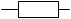
\includegraphics[scale=1]{images/resistor.jpg} \newline
$\fmm u(t) = R \cdot i(t)$ \newline
$\fmm i(t) = \frac{1}{R} \cdot u(t)$ \newline
$\fmm \underline{Z}_R = R$ \newline
&
\textbf{Kapazität C} \newline

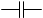
\includegraphics[scale=1]{images/condensator.jpg} \newline
$\fmm u(t) = \frac{1}{C} \int_0^t i(\tilde{t})d\tilde{t}$ \newline
$\fmm i(t) = C \cdot \frac{du(t)}{dt}$ \newline
$\fmm \underline{Z}_C = \frac{1}{j \omega C}$ \newline
Spannung springt nicht
&
\textbf{Induktivität L} \newline

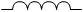
\includegraphics[scale=1]{images/inductor.jpg} \newline
$\fmm u(t) = L \cdot \frac{di(t)}{dt}$ \newline
$\fmm i(t) = \frac{1}{L} \int_0^t u(\tilde{t})d\tilde{t}$ \newline
$\fmm \underline{Z}_C = j \omega L$ \newline
Strom springt nicht

\end{tabularx} 

\subsection{Schaltvorgänge}
$\fmm u(t) = U_E + (U_A -U_E) \cdot e^{\frac{-t}{\tau}} \qquad i(t) = I_E + (I_A -I_E)
\cdot e^{\frac{-t}{\tau}} \qquad \tau = CR = \frac{L}{R}$
\textbf{Betrachte:} Zur bestimmung von R alle Quellen ausschalten und Belastung aus der
Sicht des Speicherelements betrachten.

\section{Schwingkreise}

\subsection{Freie Schwingung}

\begin{definition}
\begin{tabular}{rl|rl}
$\omega_r \rads$: & Resonanzfrequenz &
$\omega_0 \rads$: & Eigenfrequenz \\
$Q_P, Q_S$: & Güte &
$\xi = \frac{1}{2Q}$:  & Dämpfungsfaktor \\
$\alpha_{1,2}$: & \multicolumn{3}{l}{Lösungen der Charakteristischen Gleichung}
\end{tabular}
\end{definition}

\subsubsection{Ermittelung der Konstanten}

\begin{enumerate}
  \item Ermittelung der Anfangsbedingungen bei $t = 0$. $u(t)$ durch den Ansatz, dass die
  Spannung an C und der Strom an L nicht springen kann. 
  \item $\dot{u}(0)$ bestimmen aus $i_L + i_R + i_C = 0, \text{ wobei } i_C = C \cdot
  \dot{u}(0)$
  \item Ermittelung der Konstanten $\textcolor{cBlue}{U_1, U_2, \beta_u, U_a, U_b},
  \textcolor{cRed}{I_1, I_2, \beta_i, I_a, I_b}$: \newline 
  Funktion $u(t)$, bzw. $i(t)$ bei $t = 0$
  mit Anfangsbedingungen vergleichen. das selbe für $\dot{u}(t)$, bzw. $\dot{i}(t)$.
\end{enumerate}

\subsubsection{Formeln}

\begin{tabularx}{\columnwidth}{Y|Y}
  \textbf{Parallelschwingkreis} & \textbf{Seriellschwingkreis} \\
  %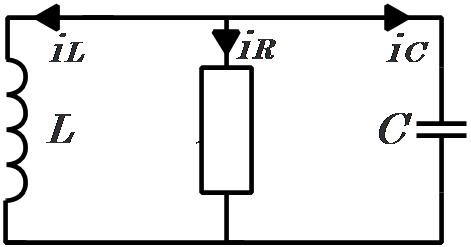
\includegraphics[scale=1]{images/psk.png} &
  %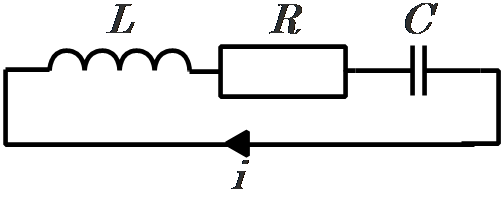
\includegraphics[scale=1]{images/ssk.png} \\
  \begin{circuitikz} [scale=0.8, transform shape]
    \draw (2,2) to [short, i=$i_L$] (0,2) to [L=$L$] (0,0) to [short] (2,0) to [short] (4,0)
      to [C=$C$] (4,2);
    \draw (2,2) to [short, i_=$i_C$] (4,2);
    \draw (2,2) to [i=$i_R$, R=$R$] (2,0);
    \draw [-latex] (2,2) to node[right, arrow head=32mm]{$i_R$}(2,1.65);
  \end{circuitikz} & 
  \begin{circuitikz} [scale=0.8, transform shape]
    \draw (0,0) to [short] (0,1) to [inductor, l_=$L$] (1.5,1) to [resistor, l_=$R$] (3,1) to [capacitor, l_=$C$] (4.5,1) to [short] (4.5,0) to [short, i=$i$] (0,0);
  \end{circuitikz}\\
  
  $\fmm \ddot{u} + \frac{1}{RC} \dot{u} + \frac{1}{LC}u = 0$ &
  $\fmm \ddot{i} + \frac{R}{L} \dot{i} + \frac{1}{LC}i = 0$ \\
  $\fmm \ddot{u} + \frac{\omega_r}{Q_P} \dot{u} + \omega_r^2 u = 0$ &
  $\fmm \ddot{i} + \frac{\omega_r}{Q_S} \dot{u} + \omega_r^2 u = 0$ \\
  $\fmm \omega_r = \frac{1}{\sqrt{LC}} \quad Q_P = R \sqrt{\frac{C}{L}}$ &
  $\fmm \omega_r = \frac{1}{\sqrt{LC}} \quad Q_S = \frac{1}{R} \sqrt{\frac{L}{C}}$  \\
  \textbf{Fall} $Q < \frac{1}{2}$: Aperiodisch $\alpha_1, \alpha_2 \in \mathbb{R}$  &
  \textbf{Fall} $Q < \frac{1}{2}$: Aperiodisch $\alpha_1, \alpha_2 \in \mathbb{R}$ \\
  $\fmm u(t) = \textcolor{cBlue}{U_1} \cdot e^{\alpha_1 t} + \textcolor{cBlue}{U_1} \cdot
  e^{\alpha_2 t}$ & 
  $\fmm i(t) = \textcolor{cRed}{I_1} \cdot e^{\alpha_1 t} + \textcolor{cRed}{I_2} \cdot
  e^{\alpha_2 t}$ \\
  $\fmm \alpha_{1,2} = -\frac{\omega_r}{2Q_P} \pm \sqrt{\frac{1}{4Q_P^2}-1}$ &
  $\fmm \alpha_{1,2} = -\frac{\omega_r}{2Q_S} \pm \sqrt{\frac{1}{4Q_S^2}-1}$ \\
  \textbf{Fall} $Q = \frac{1}{2}$: Kritisch, $\alpha_1 = \alpha_2$ &
  \textbf{Fall} $Q = \frac{1}{2}$: Kritisch, $\alpha_1 = \alpha_2$ \\
  $\fmm u(t) = (\textcolor{cBlue}{U_1} + \textcolor{cBlue}{\beta_u}) \cdot e^{\alpha t}$ &
  $\fmm i(t) = (\textcolor{cRed}{I_1} + \textcolor{cRed}{\beta_i}) \cdot e^{\alpha t}$ \\
  $\fmm \alpha_{1,2} = -\frac{\omega_r}{2Q_P} = -\omega_r$ &
  $\fmm \alpha_{1,2} = -\frac{\omega_r}{2Q_S} = -\omega_r$ \\
  \textbf{Fall} $Q > \frac{1}{2}$: Periodisch, $\alpha_1, \alpha_2 \in \mathbb{C}$ &  
  \textbf{Fall} $Q > \frac{1}{2}$: Periodisch, $\alpha_1, \alpha_2 \in \mathbb{C}$ \\
  $\fmm u(t) = e^{\frac{\omega_r}{2 Q_P} t} (\textcolor{cBlue}{U_a} \cos{\omega_0
  t} + \textcolor{cBlue}{U_b} \sin{\omega_0 t})$ &
  $\fmm i(t) = e^{\frac{\omega_r}{2 Q_S} t} (\textcolor{cRed}{I_a} \cos{\omega_0
  t} + \textcolor{cRed}{I_b} \sin{\omega_0 t})$ \\
  $\fmm \dot{u}(t = 0) = - \frac{\omega_r}{2Q_P} \textcolor{cBlue}{U_a} + \omega_0
  \textcolor{cBlue}{U_b}$ &
  $\fmm \dot{i}(t = 0) = - \frac{\omega_r}{2Q_S} \textcolor{cRed}{I_a} + \omega_0
  \textcolor{cRed}{I_b}$ \\
  $\fmm \alpha_{1,2} = -\frac{\omega_r}{2 Q_P} \pm j \omega_0$ &
  $\fmm \alpha_{1,2} = -\frac{\omega_r}{2 Q_S} \pm j \omega_0$ \\
  $\fmm \omega_0 = \omega_r \sqrt{1-\frac{1}{4 Q_P^2}}$ &
  $\fmm \omega_0 = \omega_r \sqrt{1-\frac{1}{4 Q_S^2}}$ \\
  $\omega_0 \approx \omega_r \text{ wenn } Q_P \gg \frac{1}{2})$ &
  $\omega_0 \approx \omega_r \text{ wenn } Q_S \gg \frac{1}{2})$
\end{tabularx}

\subsubsection{Kurvendiskusion}
im Folgenden wird der Faktor $y(t) = e^{-\frac{\omega_r}{2 Q}\cdot t}$ untersucht. 
\begin{itemize}
  \item $y(t = \frac{2Q}{\omega_r}) = e^{-1} \approx 0.368 = 36.8\%$
  \item nach Q Perioden: $t = Q \cdot T = \frac{2 \pi Q}{\omega_r}, y(t=\frac{2\pi
  Q}{\omega_r}) = e^{-\pi} \approx 0.0432 = 4.32\%$
\end{itemize}

\subsection{erzwungene Schwingung}
\begin{definition}
  \begin{tabular}{rl|rl}
    $\omega_1 \rads$: & untere 3dB Grenze &
    $\omega_2 \rads$: & obere 3dB Grenze \\ 
    $B \left[ \frac{1}{s} \right]$: & Bandbreite &
    $\nu$: & Verstimmung \\
    $\Omega$: & Normierte Frequenz &
    $\frac{\cn{Z}}{R} \widehat{=} \frac{\cn{Y}}{G}$: & Normierter Frequenzgang \\
  \end{tabular}
\end{definition}

\subsubsection{Formeln}

\begin{tabularx}{\columnwidth}{YY}
  $\fmm \nu = \frac{\omega}{\omega_r} - \frac{\omega_r}{\omega} = \frac{f}{f_r} -
  \frac{f_r}{f}$ &
  $\fmm \Omega = \nu \cdot Q = \left( \frac{\omega}{\omega_r} - \frac{\omega_r}{\omega}
  \right) \cdot Q$ \\
  $\fmm B = f_2 - f_1 = \frac{\omega_2 - \omega_1}{2\pi} = \frac{\omega_r}{2\pi Q}$ &
  $\omega_{1,2} = \omega_r \cdot \left(\sqrt{\frac{1}{4Q^2}+1} \mp \frac{1}{2Q}\right)$ \\
  \multicolumn{2}{c}{$\text{bei } \omega = \omega_1 \rightarrow \Omega = -1, \quad
  \text{bei } \omega = \omega_2 \rightarrow \Omega = +1$} \\ \hline
\end{tabularx}

\begin{tabularx}{\columnwidth}{Y|Y}
  \textbf{Parallelschwingkreis} & \textbf{Seriellschwingkreis} \\
  $\fmm \cn{Z} = \frac{1}{1 + j \left( \omega C - \frac{1}{\omega L} \right) \cdot R}$ &
  $\fmm \cn{Y} = \frac{G}{1 + j\left(\omega L - \frac{1}{\omega C} \cdot G \right)}$ \\
  $\fmm \frac{\cn{Z}}{R} = \frac{1}{1 + j \Omega}$ &
  $\fmm \frac{\cn{Y}}{G} = \frac{1}{1 + j \Omega}$ \\
  \textbf{bei Resonanz} $\omega = \omega_r$ &
  \textbf{bei Resonanz} $\omega = \omega_r$ \\
  $\cn{Z} = \cn{Z}_{max} = R \text{ ; } U = U_{max} = R \cdot I$ &
  $\cn{Y} = \cn{Y}_{max} = G \text{ ; } I = I_{max} = G \cdot U$ \\
  $P = P_{max} = R I^2 \text{ ; } I_L = I_C =Q_P I$ &
  $P = P_{max} = G U^2 \text{ ;} U_L = U_C =Q_S U$  \\
  $Q_L = -Q_C = Q_P \cdot P_{max}$ & 
  $Q_L = -Q_C = Q_S \cdot P_{max}$ \\
  \textbf{an 3dB-Grenzen} & \textbf{an 3dB-Grenzen} \\
  $\fmm \frac{\cn{Z}}{R} = \frac{1}{\sqrt{2}} \widehat{=} -3dB$ &
  $\fmm \frac{\cn{Y}}{G} = \frac{1}{\sqrt{2}} \widehat{=} -3dB$
\end{tabularx}

\subsubsection{Normierter Frequenzgang}
 
$$\frac{Z}{R} = \frac{1}{1+j\Omega} = \frac{1}{\sqrt{1+\Omega^2}}
\phase{-\arctan{\Omega}}, \quad \Omega = \nu \cdot Q = Q
\left(\frac{\omega}{\omega_r} - \frac{\omega_r}{\omega}\right)$$

\begin{tabularx}{\columnwidth}{YY}
  \begin{tikzpicture}
    \begin{axis}[
      xlabel=$\Omega$, 
      ylabel=$\frac{Z}{R}$,
      axis lines=middle, 
      width=0.5\columnwidth,
      height=0.35\columnwidth, 
      xmin=-4.2, 
      xmax=4.2, 
      ymin=0.1,
      ymax=1.2, 
      ytick={1},
      xtick={-3,-1,1,3},
      legend pos=north west, 
      legend style={draw=none}, 
      axis line style = {-latex}]
      
      \addplot [name path=f, color=cBlue, thick] coordinates {
        (-8.2,0.1211)(-8.1,0.1225)(-8.0,0.1240)(-7.9,0.1256)(-7.8,0.1272)(-7.7,0.1288)(-7.6,0.1305)(-7.5,0.1322)(-7.4,0.1339)(-7.3,0.1357)(-7.2,0.1376)(-7.1,0.1395)(-7.0,0.1414)(-6.9,0.1434)(-6.8,0.1455)(-6.7,0.1476)(-6.6,0.1498)(-6.5,0.1521)(-6.4,0.1544)(-6.3,0.1568)(-6.2,0.1592)(-6.1,0.1618)(-6.0,0.1644)(-5.9,0.1671)(-5.8,0.1699)(-5.7,0.1728)(-5.6,0.1758)(-5.5,0.1789)(-5.4,0.1821)(-5.3,0.1854)(-5.2,0.1888)(-5.1,0.1924)(-5.0,0.1961)(-4.9,0.2000)(-4.8,0.2040)(-4.7,0.2081)(-4.6,0.2124)(-4.5,0.2169)(-4.4,0.2216)(-4.3,0.2265)(-4.2,0.2316)(-4.1,0.2370)(-4.0,0.2425)(-3.9,0.2484)(-3.8,0.2545)(-3.7,0.2609)(-3.6,0.2676)(-3.5,0.2747)(-3.4,0.2822)(-3.3,0.2900)(-3.2,0.2983)(-3.1,0.3070)(-3.0,0.3162)(-2.9,0.3260)(-2.8,0.3363)(-2.7,0.3473)(-2.6,0.3590)(-2.5,0.3714)(-2.4,0.3846)(-2.3,0.3987)(-2.2,0.4138)(-2.1,0.4299)(-2.0,0.4472)(-1.9,0.4657)(-1.8,0.4856)(-1.7,0.5070)(-1.6,0.5300)(-1.5,0.5547)(-1.4,0.5812)(-1.3,0.6097)(-1.2,0.6402)(-1.1,0.6727)(-1.0,0.7071)(-0.9,0.7433)(-0.8,0.7809)(-0.7,0.8192)(-0.6,0.8575)(-0.5,0.8944)(-0.4,0.9285)(-0.3,0.9578)(-0.2,0.9806)(-0.1,0.9950)(0.0,1.0000)(0.1,0.9950)(0.2,0.9806)(0.3,0.9578)(0.4,0.9285)(0.5,0.8944)(0.6,0.8575)(0.7,0.8192)(0.8,0.7809)(0.9,0.7433)(1.0,0.7071)(1.1,0.6727)(1.2,0.6402)(1.3,0.6097)(1.4,0.5812)(1.5,0.5547)(1.6,0.5300)(1.7,0.5070)(1.8,0.4856)(1.9,0.4657)(2.0,0.4472)(2.1,0.4299)(2.2,0.4138)(2.3,0.3987)(2.4,0.3846)(2.5,0.3714)(2.6,0.3590)(2.7,0.3473)(2.8,0.3363)(2.9,0.3260)(3.0,0.3162)(3.1,0.3070)(3.2,0.2983)(3.3,0.2900)(3.4,0.2822)(3.5,0.2747)(3.6,0.2676)(3.7,0.2609)(3.8,0.2545)(3.9,0.2484)(4.0,0.2425)(4.1,0.2370)(4.2,0.2316)(4.3,0.2265)(4.4,0.2216)(4.5,0.2169)(4.6,0.2124)(4.7,0.2081)(4.8,0.2040)(4.9,0.2000)(5.0,0.1961)(5.1,0.1924)(5.2,0.1888)(5.3,0.1854)(5.4,0.1821)(5.5,0.1789)(5.6,0.1758)(5.7,0.1728)(5.8,0.1699)(5.9,0.1671)(6.0,0.1644)(6.1,0.1618)(6.2,0.1592)(6.3,0.1568)(6.4,0.1544)(6.5,0.1521)(6.6,0.1498)(6.7,0.1476)(6.8,0.1455)(6.9,0.1434)(7.0,0.1414)(7.1,0.1395)(7.2,0.1376)(7.3,0.1357)(7.4,0.1339)(7.5,0.1322)(7.6,0.1305)(7.7,0.1288)(7.8,0.1272)(7.9,0.1256)(8.0,0.1240)(8.1,0.1225)(8.2,0.1211)
      };
      
      \draw [dashed] (axis cs:1,0) -- (axis cs:1,0.7071);
      \draw [dashed] (axis cs:-1,0) -- (axis cs:-1,0.7071);
      \draw [dashed] (axis cs:-1,0.7071) -- (axis cs:1,0.7071);
      \filldraw [color=cBlue] (axis cs:1, 0.7071) circle (2pt);
      \filldraw [color=cBlue] (axis cs:-1, 0.7071) circle (2pt);
      \node [color=cBlue, above right] at (axis cs:1, 0.7071) {$-3dB$, $\frac{1}{\sqrt{2}}$}; 
      \node [color=cBlue, above left] at (axis cs:-1, 0.7071) {$-3dB$, $\frac{1}{\sqrt{2}}$}; 
      
    \end{axis}
  \end{tikzpicture} &
  
  \begin{tikzpicture}
    \begin{axis}[
      xlabel=$\Omega$, 
      ylabel=$\varphi$,
      axis lines=middle, 
      width=0.5\columnwidth,
      height=0.35\columnwidth, 
      xmin=-4.2, 
      xmax=4.2, 
      ymin=-1.5,
      ymax=1.5, 
      xtick={-3,-1,1,3},
      legend pos=north west, 
      legend style={draw=none}, 
      axis line style = {-latex}]
      
      \addplot [name path=f, color=cRed, thick] coordinates {
        (-8.2,1.4494)(-8.1,1.4480)(-8.0,1.4464)(-7.9,1.4449)(-7.8,1.4433)(-7.7,1.4416)(-7.6,1.4400)(-7.5,1.4382)(-7.4,1.4365)(-7.3,1.4347)(-7.2,1.4328)(-7.1,1.4309)(-7.0,1.4289)(-6.9,1.4269)(-6.8,1.4248)(-6.7,1.4226)(-6.6,1.4204)(-6.5,1.4181)(-6.4,1.4158)(-6.3,1.4134)(-6.2,1.4109)(-6.1,1.4083)(-6.0,1.4056)(-5.9,1.4029)(-5.8,1.4001)(-5.7,1.3971)(-5.6,1.3941)(-5.5,1.3909)(-5.4,1.3877)(-5.3,1.3843)(-5.2,1.3808)(-5.1,1.3772)(-5.0,1.3734)(-4.9,1.3695)(-4.8,1.3654)(-4.7,1.3612)(-4.6,1.3567)(-4.5,1.3521)(-4.4,1.3473)(-4.3,1.3423)(-4.2,1.3371)(-4.1,1.3316)(-4.0,1.3258)(-3.9,1.3198)(-3.8,1.3135)(-3.7,1.3068)(-3.6,1.2998)(-3.5,1.2925)(-3.4,1.2847)(-3.3,1.2766)(-3.2,1.2679)(-3.1,1.2588)(-3.0,1.2490)(-2.9,1.2387)(-2.8,1.2278)(-2.7,1.2161)(-2.6,1.2036)(-2.5,1.1903)(-2.4,1.1760)(-2.3,1.1607)(-2.2,1.1442)(-2.1,1.1264)(-2.0,1.1071)(-1.9,1.0863)(-1.8,1.0637)(-1.7,1.0391)(-1.6,1.0122)(-1.5,0.9828)(-1.4,0.9505)(-1.3,0.9151)(-1.2,0.8761)(-1.1,0.8330)(-1.0,0.7854)(-0.9,0.7328)(-0.8,0.6747)(-0.7,0.6107)(-0.6,0.5404)(-0.5,0.4636)(-0.4,0.3805)(-0.3,0.2915)(-0.2,0.1974)(-0.1,0.0997)(0.0,-0.0000)(0.1,-0.0997)(0.2,-0.1974)(0.3,-0.2915)(0.4,-0.3805)(0.5,-0.4636)(0.6,-0.5404)(0.7,-0.6107)(0.8,-0.6747)(0.9,-0.7328)(1.0,-0.7854)(1.1,-0.8330)(1.2,-0.8761)(1.3,-0.9151)(1.4,-0.9505)(1.5,-0.9828)(1.6,-1.0122)(1.7,-1.0391)(1.8,-1.0637)(1.9,-1.0863)(2.0,-1.1071)(2.1,-1.1264)(2.2,-1.1442)(2.3,-1.1607)(2.4,-1.1760)(2.5,-1.1903)(2.6,-1.2036)(2.7,-1.2161)(2.8,-1.2278)(2.9,-1.2387)(3.0,-1.2490)(3.1,-1.2588)(3.2,-1.2679)(3.3,-1.2766)(3.4,-1.2847)(3.5,-1.2925)(3.6,-1.2998)(3.7,-1.3068)(3.8,-1.3135)(3.9,-1.3198)(4.0,-1.3258)(4.1,-1.3316)(4.2,-1.3371)(4.3,-1.3423)(4.4,-1.3473)(4.5,-1.3521)(4.6,-1.3567)(4.7,-1.3612)(4.8,-1.3654)(4.9,-1.3695)(5.0,-1.3734)(5.1,-1.3772)(5.2,-1.3808)(5.3,-1.3843)(5.4,-1.3877)(5.5,-1.3909)(5.6,-1.3941)(5.7,-1.3971)(5.8,-1.4001)(5.9,-1.4029)(6.0,-1.4056)(6.1,-1.4083)(6.2,-1.4109)(6.3,-1.4134)(6.4,-1.4158)(6.5,-1.4181)(6.6,-1.4204)(6.7,-1.4226)(6.8,-1.4248)(6.9,-1.4269)(7.0,-1.4289)(7.1,-1.4309)(7.2,-1.4328)(7.3,-1.4347)(7.4,-1.4365)(7.5,-1.4382)(7.6,-1.4400)(7.7,-1.4416)(7.8,-1.4433)(7.9,-1.4449)(8.0,-1.4464)(8.1,-1.4480)(8.2,-1.4494)
      };
      
      \draw [dashed] (axis cs:1,0) -- (axis cs:1,-0.7854);
      \draw [dashed] (axis cs:-1,0) -- (axis cs:-1,0.7854);
      \filldraw [color=cRed] (axis cs:1, -0.7854) circle (2pt);
      \filldraw [color=cRed] (axis cs:-1, 0.7854) circle (2pt);
      \node [color=cRed, right] at (axis cs:1, -0.7854) {$-45^\circ$}; 
      \node [color=cRed, below left] at (axis cs:-1, 0.7854) {$45^\circ$}; 
      
    \end{axis}
  \end{tikzpicture}

\end{tabularx}

%$$\begin{array}{|r||c|c|c|c|c|c|c|}
%  \hline
%  \omega = & \omega_r & > \omega_r & <\omega_r & \omega_1 (-3dB) & \omega_2 (-3dB) &
%  0 & \infty \\ \hline
%  \eta = & 0 & > 0 & < 0 & -\frac{1}{Q} & \frac{1}{Q} & -\infty & +\infty \\ \hline
%\end{array}$$

\section{Reaktanz-Eintore}
\begin{definition}
  \begin{tabular}{ll|ll}
    $X = \Imag(\cn{Z})$ & Reaktanz &
    $B = \Imag(\cn{Y})$ & Suszeptanz \\
    %$X(\omega_{NS}) = 0$ & Nullstelle &
    %$X(\omega_{PS}) = \pm \infty$ & Polstelle \\
  \end{tabular}
\end{definition}

\subsection{Grundelemente}
\begin{tabularx}{\columnwidth}{Y|Y|Y|Y}
  Induktivität & Kapazität & S-Schwingkreis & P-Schwingkreis\\ 
  \adjustbox{valign=c}{\begin{circuitikz}[scale=0.8, transform shape] \draw(0,0) to
  [L](2,0); \end{circuitikz}} & 
  \adjustbox{valign=c}{\begin{circuitikz}[scale=0.8, transform shape] \draw(0,0) to
  [C](2,0); \end{circuitikz}} & 
  \adjustbox{valign=c}{\begin{circuitikz}[scale=0.8, transform shape] \draw(0,0) to
  [L](1.5,0) to [C](3,0); \end{circuitikz}}  & 
  \adjustbox{valign=c}{\begin{circuitikz}[scale=0.8, transform shape] \draw(0,0.5) to
  [-*](0.5,0.5) to (0.5,1) to [L](2.5,1) to [-*](2.5,0.5) to (3,0.5); \draw(0.5,0.5) to (0.5,0) to
  [C](2.5,0) to [-*](2.5,0.5);
  \end{circuitikz}} \\
  $X(\omega) = \omega L$ & $\fmm X(\omega) = -\frac{1}{\omega C}$ & 
  $\fmm X= \omega L - \frac{1}{\omega C}$ & $\fmm X= \frac{\omega L}{1
  - \omega^2 LC}$ \\
  \begin{tikzpicture}
    \begin{axis}[xlabel=$\omega$, ylabel = $X$, axis lines=middle,
    width=0.3\columnwidth, height=4cm, ticks=none, ymin=-1.2, ymax=1.2, xmin=0, xmax=12]
      \addplot[draw=cBlue, thick][domain=0:10]{x/10};
    \end{axis}
  \end{tikzpicture} & 
  \begin{tikzpicture}
    \begin{axis}[xlabel=$\omega$, ylabel = $X$, axis lines=middle,
    width=0.3\columnwidth, height=4cm, ticks=none, ymin=-1.2, ymax=1.2, xmin=0, xmax=12]
      \addplot[draw=cBlue, thick][domain=0:10]{-1/x};
    \end{axis}
  \end{tikzpicture} & 
  \begin{tikzpicture} 
    \begin{axis}[xlabel=$\omega$, ylabel = $X$, axis lines=middle,
    width=0.3\columnwidth, height=4cm, ytick = \empty, xtick={3.1623},
    xticklabel={\rlap{$\omega_r$}}, ymin=-1.2, ymax=1.2, xmin=0, xmax=12]
    \addplot[draw=cBlue, dashed][domain=0:10]{-1/x}; \addplot[draw=cBlue, dashed][domain=0:10]{x/10};
      \addplot[draw=cRed, thick][domain=0:10]{x/10 - 1/x};
    \end{axis}
  \end{tikzpicture} & 
  \begin{tikzpicture}
    \begin{axis}[xlabel=$\omega$, ylabel = $X$, axis lines=middle,
    width=0.35\columnwidth, height=4cm, ytick=\empty, xtick={3.1623},
    xticklabel={$\omega_r$}, ymin=-1.2, ymax=1.2, xmin=0, xmax=12] \addplot[draw=cBlue,
    dashed][domain=0:10]{-1/x}; \addplot[draw=cBlue, dashed][domain=0:10]{x/10};
      \addplot[draw=cRed, thick][domain=0:3.15]{(x/10)/(1-x*x/10)};
      \addplot[draw=cRed, thick][domain=3.17:10]{(x/10)/(1-x*x/10)};
      \draw [dotted, draw=cRed] (axis cs:3.1623, -1.1) -- (axis cs:3.1623, 1.1);
    \end{axis}
  \end{tikzpicture} \\
  
  %\textbf{Nullstellen:} & & & \\
  \textbf{Nullstellen}: $\omega = 0$ & $\omega \rightarrow \infty$ & $\fmm \omega =
  \omega_r = \frac{1}{\sqrt{LC}}$ & $\omega = 0, \omega \rightarrow \infty$ \\
  %\textbf{Polstellen:} & & & \\
  \textbf{Polstellen}: $\omega \rightarrow \infty$ & $\omega = 0$ & $\omega \rightarrow 0,
  \omega \rightarrow \infty$ & $\omega = \omega_r = \frac{1}{\sqrt{LC}}$
  
  
\end{tabularx}

\subsection{Eigenschaften}

$\fmm \cn{Z}(j\omega) = \frac{a_n (j \omega)^n +
a_{n-2}(j\omega)^{n-2} + a_{n-4} (j \omega)^{n-4}}{b_m (j \omega)^m +
b_{m-2}(j\omega)^{m-2} + b_{m-4} (j \omega)^{m-4}} = \frac{P_n(j\omega)}{Q_m(j \omega)}$ 

\begin{itemize}
  \item $\abs{n - m} = 1$: Im Zähler und im Nenner kommen nie dieselben Potenzen vor. 
  \item Den Polynomen $P_n(j\omega)$ und $Q_n(j\omega)$ fehlen keine Koeffizienten.
  \item Die Anzahl der Elemente entspicht der Anzahl endlicher Nullstellen und Polstellen.
  \item Die Ableitung der Funktion $\cn{Z}(j\omega)$ ist immer positiv, d.H $\cn{Z}$ ist
  monoton Steigend.
\end{itemize}

\subsection{Minimum-Reaktanz-Eintore MRET}
\begin{tabularx}{\columnwidth}{XX}
  Wenn ein \textbf{Kreis} aus lauter L oder C vorhanden ist, kann ein L (bzw. C)
  weggelassen (unterbrochen) werden. klemmen bleiben geöffnet!& 
  \adjustbox{valign=t}{\begin{circuitikz}[scale=0.5, transform shape]
    \draw(-0.5,0.4) to (0,0) to [L, *-*] (3,0) to (3.6,0.2);
    \draw(3.6,2.8) to (3,3) to [L, *-] (3,0) to (2.7, -0.5);
    \draw(-0.3,2.4) to (0,3) to [L, *-] (3,3) to (3.4,3.4);
    \draw(-0.5,3.1) to (0,3) to [L] (0,0) to (-0.5,-0.4);
    \draw(0,3) to [C] (3,0);
    \draw[dotted, thick, draw=cRed](1.5,1.5) circle[radius=1.2];
    \draw[thick, draw=cRed](2.2, 3.3) to (2.8,2.7);
    \draw[thick, draw=cRed](2.2, 2.7) to (2.8,3.3);
    
    \draw[thick, -latex, draw=black](4, 1.5) -- (5,1.5);
    
    \draw(5.5,0.4) to (6,0) to [L, *-*] (9,0) to (9.6,0.2);
    \draw(9.6,2.8) to (9,3) to [L, *-] (9,0) to (8.7, -0.5);
    \draw(5.3,2.4) to (6,3);
    \draw(9,3) to (9.4,3.4);
    \draw(5.5,3.1) to (6,3) to [L, *-] (6,0) to (5.5,-0.4);
    \draw(6,3) to [C] (9,0);
  \end{circuitikz}} \\
  Ein \textbf{Trennbündel}, wie auf der Grafik angezeigt, darf nur L oder C-Elemente
  schneiden. Sobald ein Trennbündel gefunden wurde, ein Element kurzgeschlossen werden.
  Die Klemmen müssen geschlossen werden!& 
  \adjustbox{valign=t}{\begin{circuitikz}[scale=0.5,transform shape]
    \draw(0, 0) to [C, *-*] (3,0) to (3.5,0.2);
    \draw(3,0) to (3.2,-0.5);
    \draw(-0.5,3.8) to (0,4) to [C, *-*] (0,2) to [L](0,0);
    \draw(0,2) to [C, -*] (3,2) to (2.7,2.4);
    \draw(3,2) to (3.5, 1.8);
    \draw[dotted, thick, draw=cRed](0,1) circle (2);
    \draw[thick, draw=cRed](2.3,2) arc (0:180:0.8);
    
    \draw[thick, -latex, draw=black](4,2) -- (5,2);
    
    \draw(6, 0) to [C, *-*] (9,0) to (9.5,0.2);
    \draw(9,0) to (9.2,-0.5);
    \draw(5.5,3.8) to (6,4) to [C, *-*] (6,2) to [L](6,0);
    \draw(6,2) to (9,2) to (8.7,2.4);
    \draw(9,2) to (9.5, 1.8);
  \end{circuitikz}}
\end{tabularx}

\subsection{Bestimmung des RET-Types}
\footnotesize\begin{tabular}{c|c|c|c|c|c|c|c}
  Typ & $X(\omega)$ & $\omega = 0$ & $\omega \rightarrow \infty$ & L-Kr. & L-Tb. & 
  C-Kr. & C-Tb. \\ \hline
  \textbf{L} &
  \adjustbox{valign=c}{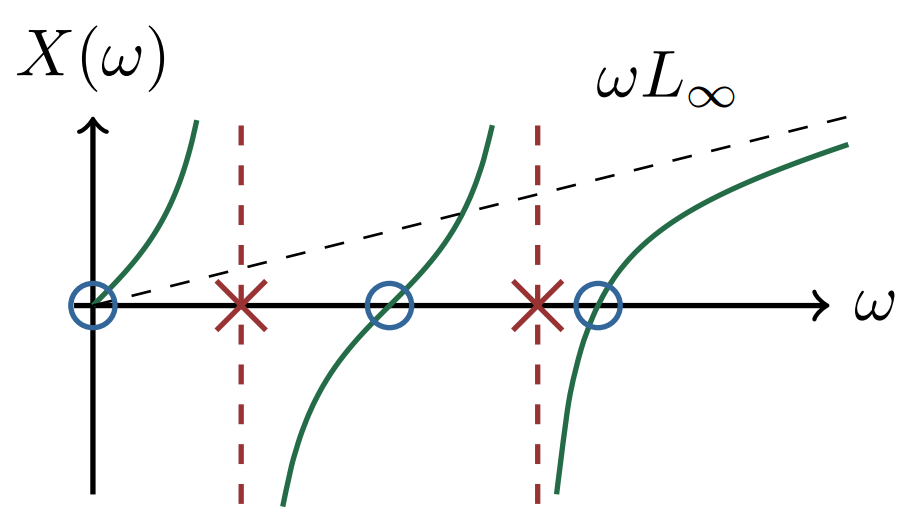
\includegraphics[scale=0.09]{images/RetTypL}}
  & \nullstelle & \pol & \symtrue & \symtrue & \symfalse & \symfalse \\
  \textbf{C} &
  \adjustbox{valign=c}{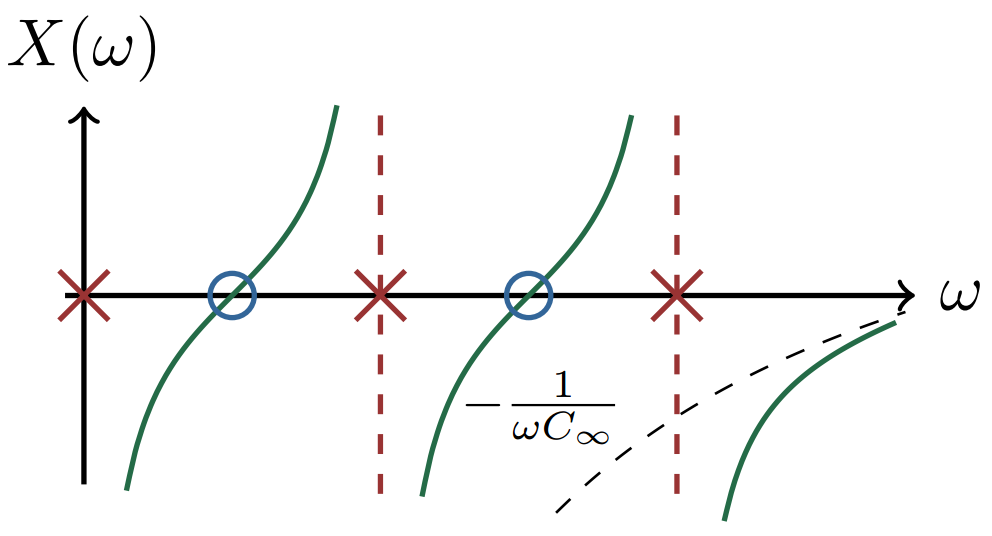
\includegraphics[scale=0.09]{images/RetTypC}}
  & \pol & \nullstelle & \symfalse & \symfalse & \symtrue & \symtrue \\
  \textbf{S} & 
  \adjustbox{valign=c}{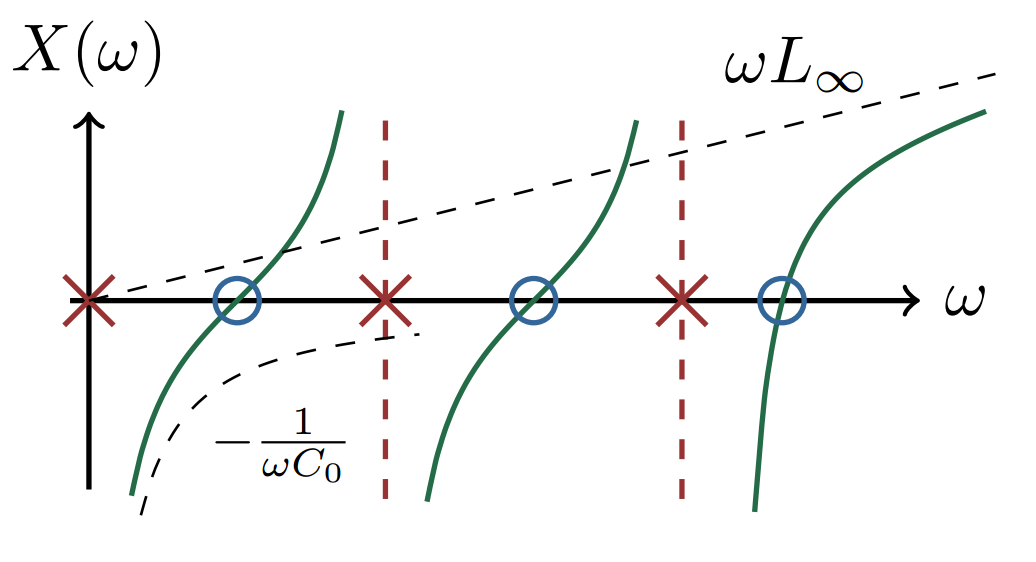
\includegraphics[scale=0.09]{images/RetTypS}}
  & \pol & \pol & \symfalse & \symtrue & \symfalse & \symtrue \\
  \textbf{P} &
  \adjustbox{valign=c}{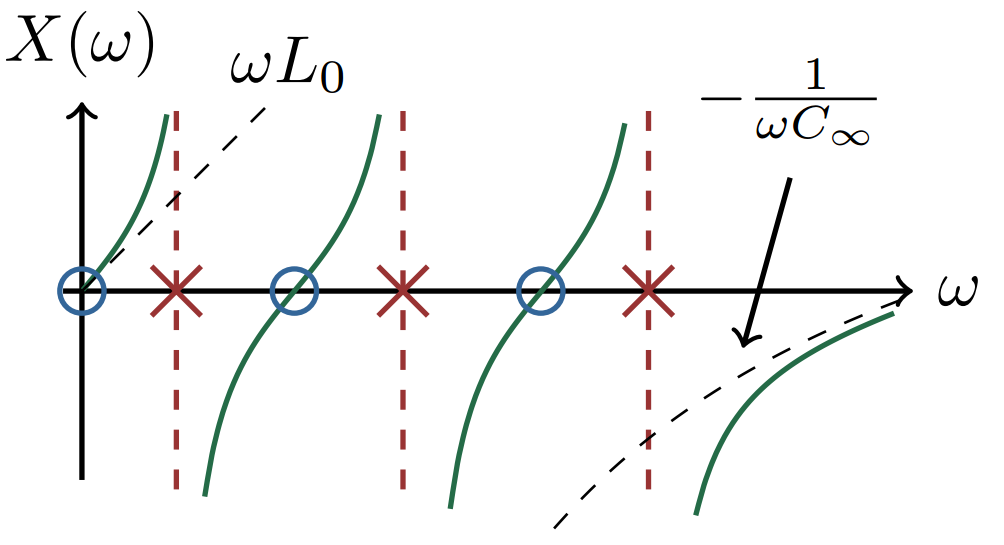
\includegraphics[scale=0.09]{images/RetTypP}}
  & \nullstelle & \nullstelle & \symtrue & \symfalse & \symtrue & \symfalse\\
\end{tabular}

\subsection{RET-Synthese}

\subsubsection{Mittels Partialbruchzerlegung}
\begin{tabular}{ll}
1.~Impedanz- oder Admitanzfunktion & $\fmm \cn{F}(s) = \frac{2s^6 + 22s^4 + 58s^2 + 48}{3s^5 + 21s^3 + 30s}$ \\
2.~PBZ bilden \& koeffizienten ermitteln & $\fmm \cn{F}(s) = \frac{2s}{3} + \frac{A}{3s} + \frac{Bs}{s^2+1} + \frac{Cs}{s^2+5}$ \\
 & $\text{mit } A = \frac{24}{5}, \quad B = \frac{8}{9}, \quad C = \frac{8}{45}$ \\
3.~Nach Netzwerkelementen umformen & $\fmm \cn{F}(s) = \frac{2}{3}s + \frac{1}{\frac{15}{24}s} + \frac{1}{\frac{9}{8}s + \frac{1}{\frac{4}{9}s}} + \frac{1}{\frac{45}{8}s + \frac{1}{\frac{8}{255}s}}$
\end{tabular}

\subsubsection{Mittels Kettenbruchzerlegung}
\begin{mtabular}{ll}
1.~Voraussetzung: Unecht gebrochen & $\fmm \cn{F}(s) = \frac{2s^6 + 22s^4 + 58s^2 + 48}{3s^5 + 21s^3 + 30s}$ \\
2.~Polynomdivision ausführen & $\fmm \cn{F}(s) = \frac{2}{3}s \cdot + \frac{8s^4 + 48s^2 + 48}{3s^5 + 21s^3 + 30s}$ \\
3.~mit Kehrwert des Rests bei 2. fortfahren & $\fmm \cn{F}_1(s) = \frac{3s^5 + 21s^3 + 30s}{8s^4 + 48s^2 + 48}$ \\
\multicolumn{2}{l}{4.~Abgespaltete Werte Seriell und Parallel (je nach Bedeutung von $\cn{F}_n$) sind die Elemente.}
\end{mtabular}

\subsection{Äquivalenz}
\begin{enumerate}
  \item Gegebenees RET übersichtlich aufzeichnen
  \item In das RET zusätzlich L- bzw. C-Elemente so einfügen, dass L- bzw. C-Kreise oder Trennbündel entstehen.
  \item Durch Weglassen / Kurzschliessen von alten RET-Eementen das erweiterte RET auf ein MRET zurückführen.
  \item Impedanzfunktion des alten RET und des MRET berechnen und die unbekannten Elemente durch Koeffizientenvergleich bestimmen.
\end{enumerate}

\section{Zweitore} 

\begin{tabular}{p{0.3\columnwidth}p{0.65\columnwidth}}
  \begin{tabular}{l}
    \begin{circuitikz}[scale=0.8, transform shape]
  
      %Primärseite
      \draw (0,2) to [short, i=$\cn{I}_1$, o-] (1,2);
      \draw (0,0) to [short, o-] (1,0);
      \draw[-latex,shorten >=2mm, shorten <=2mm,in=120, out=240] (0,2) to node[right] {$\cn{U}_1$} (0,0);
      
      %2tor
      \draw(1,-0.5) to [short] (1,2.5) to [short] (3, 2.5) to [short] (3,-0.5) to [short] (1,-0.5);
      \draw(2,1) node{2-Tor};
    
      %Sekundärseite
      \draw (4,2) to [short, i=$\cn{I}_2$, o-] (3,2);
      \draw (4,0) to [short, o-] (3,0);
      \draw[-latex,shorten >=2mm, shorten <=2mm,out=300, in=60] (4,2) to node[left] {$\cn{U}_2$} (4,0);
    
      \draw[draw=none] (4.5,1) to (5.5,1);
    
    \end{circuitikz}  
  \end{tabular} &
  \begin{tabular}{p{0.63\columnwidth}}
    \begin{itemize}
      \item \textbf{Reziprok}: Speist man ein reziprokes Zweitor aus einer Quelle mit Innenwiederstand 
      $\cn{Z}_0$ und belastet es am Ausgang mit der selben Impedanz $\cn{Z}_0$, so ist es für die 
      Kenngrössen gleichgültig, in welcher Richtung das Zweitor betrieben wird.
      \item \textbf{Richtsymmetrie}: Beide Tore können elektrisch beim Umtauschen nicht unterschieden 
      werden.
      \item \textbf{Erdsymmetrie}: Werdem die beiden Eingangsanschlüsse, so wie die 
      Ausgangsanschlüsse, separat vertauscht, ist kein Unterschied von Aussen erkennbar.
    \end{itemize}
  \end{tabular} \\
\end{tabular}

 
\subsection{Matrizen}
\begin{tabular}{lll}
  \textbf{Form} & \textbf{Vierpolgleichung} & \textbf{Berechnung} \\
  \toprule
  \textbf{Impedanz} & 
  $\begin{mat1} \cn{U}_1 \\ \cn{U}_2 \end{mat1} = [Z] \begin{mat1}\cn{I}_1\\ \cn{I}_2\end{mat1}$ &
  $\fmm [\cn{Z}] = \begin{mat2}
    \cn{Z}_{11} = \left. \frac{\cn{U}_1}{\cn{I}_1} \right|_{\cn{I}_2 = 0} & 
    \cn{Z}_{12} = \left. \frac{\cn{U}_1}{\cn{I}_2} \right|_{\cn{I}_1 = 0} \\
    \cn{Z}_{21} = \left. \frac{\cn{U}_2}{\cn{I}_1} \right|_{\cn{I}_2 = 0} & 
    \cn{Z}_{22} = \left. \frac{\cn{U}_2}{\cn{I}_2} \right|_{\cn{I}_1 = 0}   
  \end{mat2}$ \\
  \midrule
  \textbf{Admitanz} & 
  $\begin{mat1} \cn{I}_1 \\ \cn{I}_2 \end{mat1} = [Y] \begin{mat1}\cn{U}_1\\ \cn{U}_2\end{mat1}$ &
  $\fmm [\cn{Y}] = \begin{mat2}
    \cn{Y}_{11} = \left. \frac{\cn{I}_1}{\cn{U}_1} \right|_{\cn{U}_2 = 0} & 
    \cn{Y}_{12} = \left. \frac{\cn{I}_1}{\cn{U}_2} \right|_{\cn{U}_1 = 0} \\
    \cn{Y}_{21} = \left. \frac{\cn{I}_2}{\cn{U}_1} \right|_{\cn{U}_2 = 0} & 
    \cn{Y}_{22} = \left. \frac{\cn{I}_2}{\cn{U}_2} \right|_{\cn{U}_1 = 0}   
  \end{mat2}$ \\
  \midrule
  \textbf{Ketten} & 
  $\begin{mat1} \cn{U}_1 \\ \cn{I}_1 \end{mat1} = [A] \begin{mat1}\cn{U}_2\\ -\cn{I}_2\end{mat1}$ &
  $\fmm [\cn{A}] = \begin{mat2}
    \cn{A}_{11} = \left. \frac{\cn{U}_1}{\cn{U}_2} \right|_{\cn{I}_2 = 0} & 
    \cn{A}_{12} = \left. \frac{\cn{U}_1}{-\cn{I}_2} \right|_{\cn{U}_2 = 0} \\
    \cn{A}_{21} = \left. \frac{\cn{I}_1}{\cn{U}_2} \right|_{\cn{I}_2 = 0} & 
    \cn{A}_{22} = \left. \frac{\cn{I}_1}{-\cn{I}_2} \right|_{\cn{U}_2 = 0}   
  \end{mat2}$ \\
  \midrule
  \textbf{Hybrid} & 
  $\begin{mat1} \cn{U}_1 \\ \cn{I}_2 \end{mat1} = [H] \begin{mat1}\cn{I}_1\\ \cn{U}_2\end{mat1}$ &
  $\fmm [\cn{H}] = \begin{mat2}
    \cn{H}_{11} = \left. \frac{\cn{U}_1}{\cn{I}_1} \right|_{\cn{U}_2 = 0} & 
    \cn{H}_{12} = \left. \frac{\cn{U}_1}{\cn{U}_2} \right|_{\cn{I}_1 = 0} \\
    \cn{H}_{21} = \left. \frac{\cn{I}_2}{\cn{I}_1} \right|_{\cn{U}_2 = 0} & 
    \cn{H}_{22} = \left. \frac{\cn{I}_2}{\cn{U}_2} \right|_{\cn{I}_1 = 0}   
  \end{mat2}$ \\
\end{tabular}


\begin{center}
\begin{tabular}{lllll}
 & \multicolumn{4}{c}{\textbf{Koeffizientenbeziehungen}} \\
 \toprule
 \textbf{reziprok} & $\cn{Z}_{12} = \cn{Z}_{21}$, & $\cn{Y}_{12} = \cn{Y}_{21}$, & $\det[A] = 1$, & $\cn{H}_{12} = - \cn{H}_{21}$ \\
 \midrule
 \textbf{symmetrisch} & $\cn{Z}_{12} = \cn{Z}_{21}$, & $\cn{Y}_{12} = \cn{Y}_{21}$, & $\det[A] = 1$, & $\cn{H}_{12} = - \cn{H}_{21}$ \\
 & $\cn{Z}_{11} = \cn{Z}_{22}$, & $\cn{Y}_{11} = \cn{Y}_{22}$, & $\cn{A}_{11} = \cn{A}_{22}$, & $\det[H] = 1$ \\
\end{tabular}
\end{center}

\subsection{Leerlauf und Kurzschluss am Zweitor}

Bei einer \cdef{Kurzschlussimpedanz $\cn{Z_{1k}}$, $\cn{Z_{2k}}$} wird die jeweils
gegenüberliegende Seite kurzgeschlossen. Bei den \cdef{Leerlaufimpedanzen $\cn{Z_{1l}}$, $\cn{Z_{2l}}$} 

$$\begin{array}{>{\fmm}c >{\fmm}c >{\fmm}c >{\fmm}c >{\fmm}c}
  & [\cn{A}] & [\cn{Z}] & [\cn{Y}] & [\cn{H}] \\
  \toprule
  \cn{Z_{1k}} = & 
  \frac{\cn{A}_{12}}{\cn{A}_{11}} & 
  \frac{\det{[\cn{Z}]}}{\cn{Z}_{22}} &
  \frac{1}{\cn{Y}_{11}} &
  \cn{H}_{11} \\
  \midrule
  \cn{Z_{2k}} = & \frac{\cn{A}_{12}}{\cn{A}_{11}} &
  \frac{\det{[\cn{Z}]}}{\cn{Z}_{11}} &
  \frac{1}{\cn{Y}_{22}} &
  \frac{\cn{H}_{11}}{\det{[\cn{H}]}} \\
  \midrule
  \cn{Z}_{1l} = &
  \frac{\cn{A}_{11}}{\cn{A}_{21}} &
  \cn{Z_{11}} &
  \frac{\cn{Y}_{22}}{\det{[\cn{Y}]}} &
  \frac{1}{\cn{H}_{22}} \\
  \midrule
  \cn{Z}_{2l} = & \frac{\cn{A}_{22}}{\cn{A}_{21}} &
  \cn{Z}_{22} &
  \frac{\cn{Y}_{11}}{\det{[\cn{Y}]}} &
  \frac{1}{\cn{H}_{22}} \\
\end{array}$$

\subsection{Ersatzschaltungen}
\begin{tabular}{ll}
  \begin{tabular}{l}
    \begin{circuitikz} [scale=0.8, transform shape]
      \draw (0,2) to [short, i=$\cn{I}_1$, *-] (1,2) to [resistor, l_=$\cn{Z}_{11}$] (3,2);
      \draw (0,0) to [short, *-](3,0) to [voltage source] (3,2);
      \draw [-latex] (4.4,1) to node[above]{$\cn{Z}_{12} \cdot \cn{I}_2$} (3.4,1);
      \draw[-latex,shorten >=2mm, shorten <=2mm,in=120, out=240] (0,2) to node[right] {$\cn{U}_1$} (0,0);
         
      \draw (9,2) to [short, i=$\cn{I}_1$, *-] (8,2) to [resistor, l^=$\cn{Z}_{22}$] (6,2);
      \draw (9,0) to [short, *-](6,0) to [voltage source] (6,2);
      \draw [-latex] (4.6,1) to node[above]{$\cn{Z}_{21} \cdot \cn{I}_1$} (5.6,1);
      \draw[-latex,shorten >=2mm, shorten <=2mm,out=300, in=60] (9,2) to node[left] {$\cn{U}_2$} (9,0);
    \end{circuitikz}
  \end{tabular} &
  \begin{tabular}{l}
    \textbf{Z-Ersatzschaltung}: \\
    $\cn{U}_1 = \cn{Z}_{11} \cdot \cn{I}_1 + \cn{Z}_{12} \cdot \cn{I}_2$ \\
    $\cn{U}_2 = \cn{Z}_{21} \cdot \cn{I}_1 + \cn{Z}_{22} \cdot \cn{I}_2$ \\
  \end{tabular} \\
  
  %\midrule
  
  \begin{tabular}{l}
    \begin{circuitikz} [scale=0.8, transform shape]
      \draw (0,2) to [short, i=$\cn{I}_1$, *-] (1,2) to [short] (3,2) to [I] (3,0) to [short, -*](0,0);
      \draw (2,2) to [resistor, l_={$\cn{Y}_{11}$}] (2,0);
      \draw [-latex] (4.4,1) to node[above]{$\cn{Y}_{12} \cdot \cn{U}_2$} (3.4,1);
      \draw[-latex,shorten >=2mm, shorten <=2mm,in=120, out=240] (0,2) to node[right] {$\cn{U}_1$} (0,0);
         
      \draw (9,2) to [short, i=$\cn{I}_1$, *-] (8,2) to [short] (6,2) to [I] (6,0) to [short, -*](9,0);
      \draw (7,2) to [resistor, l={$\cn{Y}_{22}$}] (7,0);
      \draw [-latex] (4.6,1) to node[above]{$\cn{Y}_{21} \cdot \cn{U}_1$} (5.6,1);
      \draw[-latex,shorten >=2mm, shorten <=2mm,out=300, in=60] (9,2) to node[left] {$\cn{U}_2$} (9,0);
    \end{circuitikz}
  \end{tabular} &
  \begin{tabular}{l}
    \textbf{Y-Ersatzschaltung}: \\
    $\cn{I}_1 = \cn{Y}_{11} \cdot \cn{U}_1 + \cn{Y}_{12} \cdot \cn{U}_2$ \\
    $\cn{I}_2 = \cn{Y}_{21} \cdot \cn{U}_1 + \cn{Y}_{22} \cdot \cn{U}_2$ \\
  \end{tabular} \\
  
  %\midrule
  
  \begin{tabular}{l}
    \begin{circuitikz} [scale=0.8, transform shape]
      \draw (0,2) to [short, i=$\cn{I}_1$, *-] (1,2) to [resistor, l_={$\cn{H}_{11}$}] (3,2);
      \draw (0,0) to [short, *-](3,0) to [voltage source] (3,2);
      \draw [-latex] (4.4,1) to node[above]{$\cn{H}_{12} \cdot \cn{U}_2$} (3.4,1);
      \draw[-latex,shorten >=2mm, shorten <=2mm,in=120, out=240] (0,2) to node[right] {$\cn{U}_1$} (0,0);
         
      \draw (9,2) to [short, i=$\cn{I}_1$, *-] (8,2) to [short] (6,2) to [I] (6,0) to [short, -*](9,0);
      \draw (7,2) to [resistor, l={$\frac{1}{\cn{H}_{22}}$}] (7,0);
      \draw [-latex] (4.6,1) to node[above]{$\cn{H}_{21} \cdot \cn{I}_1$} (5.6,1);
      \draw[-latex,shorten >=2mm, shorten <=2mm,out=300, in=60] (9,2) to node[left] {$\cn{U}_2$} (9,0);
    \end{circuitikz}
  \end{tabular} &
  \begin{tabular}{l}
    \textbf{H-Ersatzschaltung}: \\
    $\cn{U}_1 = \cn{H}_{11} \cdot \cn{I}_1 + \cn{H}_{12} \cdot \cn{U}_2$ \\
    $\cn{I}_2 = \cn{H}_{21} \cdot \cn{I}_1 + \cn{H}_{22} \cdot \cn{U}_2$ \\
  \end{tabular} \\
\end{tabular}

\subsection{Zusammenschaltung von Zweitoren}

\begin{tabular}{cc}
  \begin{tabular}{c}
    \begin{circuitikz} [scale=0.8, transform shape]
      \draw (1.75,0.5) node[zweitor] (ZT1) {$[\cn{A}']$};
      \draw (4.25,0.5) node[zweitor] (ZT2) {$[\cn{A}'']$};
      
      \draw (0,0) to [short, o-] (ZT1.B1);
      \draw (0,1) to [short, i = $\cn{I}_1$, o-] (ZT1.A1);
      \draw (ZT1.A2) to [short] (ZT2.A1);
      \draw (ZT1.B2) to [short] (ZT2.B1);
      \draw (6,1) to [short, i = $\cn{I}_2$, o-] (ZT2.A2);
      \draw (ZT2.B2) to [short, -o] (6,0);
      
      \draw[-latex,shorten >=2mm, shorten <=2mm,in=90, out=270] (0,1.1) to node[right] {$\cn{U}_1$} (0,-0.1);
      \draw[-latex,shorten >=2mm, shorten <=2mm,out=270, in=90] (6,1.1) to node[right] {$\cn{U}_2$} (6,-0.1);
          
    \end{circuitikz} \\
    $[\cn{A}] = [\cn{A}'] \cdot [\cn{A}'']$
  \end{tabular} & 
  
  \begin{tabular}{c}
    \begin{circuitikz} [scale=0.8, transform shape]
      \draw (2.75, 2.5) node[zweitor] (ZT1) {$[\cn{Z}']$};
      \draw (2.75, 0.5) node[zweitor] (ZT2) {$[\cn{Z}'']$};
      
      \draw (0,3) to [short, i=$\cn{I}_1$, o-] (ZT1.A1);
      \draw (0,0) to [short, o-] (ZT2.B1);
      \draw (ZT1.B1) to [short] +(-1, 0) to [short] + (0, -1) to [short] (ZT2.A1);
      \draw (ZT1.B2) to [short] +(1, 0) to [short] + (0, -1) to [short] (ZT2.A2);
      \draw (5.5,3) to [short, i = $\cn{I}_2$, o-] (ZT1.A2);
      \draw (5.5,0) to [short, o-] (ZT2.B2); 
      
      \draw[-latex,shorten >=2mm, shorten <=2mm,in=120, out=240] (0,3) to node[right] {$\cn{U}_1$} (0,0);
      \draw[-latex,shorten >=2mm, shorten <=2mm,out=300, in=60] (5.5,3) to node[left] {$\cn{U}_2$} (5.5,0);
       
      
    \end{circuitikz} \\
    $[\cn{Z}] = [\cn{Z}'] + [\cn{Z}'']$ 
  \end{tabular} \\
  
  \begin{tabular}{c}
    \begin{circuitikz} [scale=0.8, transform shape]
      \draw (2.75, 2.5) node[zweitor] (ZT1) {$[\cn{Y}']$};
      \draw (2.75, 0.5) node[zweitor] (ZT2) {$[\cn{Y}'']$};
          
      \draw (0,2.5) to [short, i=$\cn{I}_1$, o-*] (1,2.5);
      \draw (0,0.5) to [short, o-*] (1.5,0.5);
      \draw (ZT1.A1) to [short] (1,3) to [short] (1,1) to [short] (ZT2.A1);
      \draw (ZT1.B1) to [short] (1.5,2) to [short] (1.5,0) to [short] (ZT2.B1);
      
      \draw (5.5,2.5) to [short, i=$\cn{I}_2$, o-*] (4.5, 2.5);
      \draw(5.5,0.5) to [short, o-*] (4, 0.5);
      \draw (ZT1.A2) to [short] (4.5,3) to [short] (4.5,1) to [short] (ZT2.A2);
      \draw (ZT1.B2) to [short] (4,2) to [short] (4,0) to [short] (ZT2.B2);
      
      \draw[-latex,shorten >=2mm, shorten <=2mm,in=120, out=240] (0,2.5) to node[right] {$\cn{U}_1$} (0,0.5);
      \draw[-latex,shorten >=2mm, shorten <=2mm,out=300, in=60] (5.5,2.5) to node[left] {$\cn{U}_2$} (5.5,0.5);
       
    \end{circuitikz} \\
    $[\cn{Y}] = [\cn{Y}'] \cdot [\cn{Y}'']$
  \end{tabular} & 
  
  \begin{tabular}{c}
    \begin{circuitikz} [scale=0.8, transform shape]
      \draw (2.75, 2.5) node[zweitor] (ZT1) {$[\cn{H}']$};
      \draw (2.75, 0.5) node[zweitor] (ZT2) {$[\cn{H}'']$};
      
      \draw (0,3) to [short, i=$\cn{I}_1$, o-] (ZT1.A1);
      \draw (0,0) to [short, o-] (ZT2.B1);
      \draw (ZT1.B1) to [short] +(-1, 0) to [short] + (0, -1) to [short] (ZT2.A1);
      
      \draw (5.5,2.5) to [short, i=$\cn{I}_2$, o-*] (4.5, 2.5);
      \draw(5.5,0.5) to [short, o-*] (4, 0.5);
      \draw (ZT1.A2) to [short] (4.5,3) to [short] (4.5,1) to [short] (ZT2.A2);
      \draw (ZT1.B2) to [short] (4,2) to [short] (4,0) to [short] (ZT2.B2);
      
      \draw[-latex,shorten >=2mm, shorten <=2mm,in=120, out=240] (0,3) to node[right] {$\cn{U}_1$} (0,0);
      \draw[-latex,shorten >=2mm, shorten <=2mm,out=300, in=60] (5.5,2.5) to node[left] {$\cn{U}_2$} (5.5,0.5);
           
    \end{circuitikz} \\
    $[\cn{H}] = [\cn{H}'] + [\cn{H}'']$ 
  \end{tabular} \\
\end{tabular}

\section{Netzwerke und Systeme}
\subsection{Duale Netzwerke}

\begin{enumerate}
  \item Zählrichtung Festlegen (z.B: im Uhrzeigersinn $\rightarrow$ Pfeile nach Innen).
  \item In jede Netzwerkmasche einen Knoten für das duale Netzwerk setzen
  \item Alle Elemente durchschneiden und mit dualen Elementen den benachbarten Knoten verbinden
  \item Zählrichtungen übertragen (wie zuvor Festgelegt)
  \item Dualfaktoren wählen:
\end{enumerate}

$$R' = \frac{D^2}{R}, \quad L' = D^2 C, \quad C' = \frac{L}{D^2}, \quad \cn{U}' = D \cn{I}, \quad \cn{I}' = \frac{\cn{U}}{D}$$

\subsection{Netzwerkfunktionen}

\begin{mtabular}{rp{0.7\columnwidth}}
Polynom-Darstellung: & $ \fmm \cn{F}(s) = K \cdot \frac{s^n + a_{n-1} s^{n-1} + \ldots + a_1 s + a_0}{s^m + b_{m-1} s^{m-1} + \ldots + b_1 s + b_0} = K \frac{P_n(s)}{Q_m(s)}$ \\
Produktform & $\fmm \cn{F}(s) = k \cdot \frac{(s - n_1)(s - n_2) \ldots (s - n_n)}{(s - p_1)(s-p_2) \ldots (s - p_m)}$ \\
Norm. Produktform & Es kommen nur Faktoren $(s)$ , $(1 + a s)$ und $(1 + bs + cs^2)$ vor. \newline 
                    Alle Konstanten sind reell\\
Partialbruchform: & $\fmm \cn{F}(s) = B_0 + B_1 s + \frac{K_1}{s - p_1} + \frac{K_2}{s - p_2} + \ldots + \frac{K_n}{s - p_n}$ \\

\end{mtabular}

\subsection{Pol und Ortskurve des Parallelschwingkreis}



\begin{tabular}{ll}
  \begin{tabular}{ll} 
    \multicolumn{2}{l}{$ \fmm \cn{Z}(s) = \frac{sL}{s^2 LC + s \frac{L}{R} + 1 } = \omega_r^2 \frac{sL}{s^2 + s \frac{\omega_r}{Q} + \omega_r^2} $} \\
    {\color{cRed}    $Q \ll \frac{1}{2}$} &
    {\color{cRed}    $s_{1,2} \approx 0,-\infty$} \\
    {\color{cBlue}   $Q < \frac{1}{2}$} &
    {\color{cBlue}   $s_{1,2} = -\frac{\omega_r}{2Q} \pm \omega_r \sqrt{\frac{1}{4Q^2}-1}$} \\
    {\color{cGreen}  $Q = \frac{1}{2}$} &
    {\color{cGreen}  $s_{1,2} = -\omega_r$} \\ 
    {\color{cOrange} $Q > \frac{1}{2}$} &
    {\color{cOrange} $s_{1,2} = -\frac{\omega_r}{2Q} \pm j \omega_r \sqrt{1-\frac{1}{4Q^2}}$} \\
    {\color{black}   $Q \gg \frac{1}{2}$} &
    {\color{black}   $s_{1,2} \approx \pm j\omega_r$}\\
  \end{tabular} &
  \begin{tabular}{ll}
    \begin{tikzpicture} [scale=0.9, transform shape]
      \begin{axis} [
        width= 0.5\columnwidth,
        height=0.5\columnwidth,
        xlabel={$\sigma$},
        ylabel={$j \omega$},
        axis lines=middle,
        xmin = -2,
        xmax = 0.4,
        ymin = -1.2,
        ymax = 1.2,
        xtick={-1},
        xticklabels={$-\omega_r$},
        every x tick label/.style={xshift=-4mm},
        ytick={-1,1},
        yticklabels={$-j \omega_r$, $j \omega_r$},
        %ytickstyle ={y tick label style={right}},
        every y tick label/.style={right, xshift=1mm},
        every axis y label/.style={
          at={(ticklabel* cs:1)},
          anchor=south,
        },
        clip=false,
      ]
        
        \draw (axis cs:-1.8,-0.05) -- (axis cs:-1.78,0.05);
        \draw (axis cs:-1.78,-0.05) -- (axis cs:-1.76,0.05);
        
        \draw [cRed] (axis cs:0,0) node {$\times$};
        \draw [cRed] (axis cs:-1.95,0) node {$\times$};
        \draw [cGreen] (axis cs:-1.01,0) node {$\times$};
        \draw [cGreen] (axis cs:-0.99,0) node {$\times$};
        \draw [black] (axis cs:0,1) node {$\times$};
        \draw [black] (axis cs:0,-1) node {$\times$};
        
        \draw [thick, cBlue] (axis cs:0,0) -- (axis cs:-1.95,0);
        \draw [thick, cOrange] (axis cs:0,1) arc (90:270:{transformdirectionx(1)});
        
        %arrows
        \draw [>=latex, ->, cRed,   shorten >=1mm] (axis cs:0.2, -0.4) node[below right] {$Q \rightarrow 0$} -- (axis cs:0,0);
        \draw [>=latex, ->, cRed,   shorten >=1mm] (axis cs:-1.75,-0.4) node[below right] {$Q \rightarrow 0$} -- (axis cs:-1.95,0);
        \draw [>=latex, ->, cGreen, shorten >=1mm] (axis cs:-0.6, -0.2) node[below right] {$Q = \frac{1}{2}$}  -- (axis cs:-1,0);
        \draw [>=latex, ->, cBlue]   (axis cs:-0.3,0.1) -- node[above] {Q} (axis cs:-0.7,0.1);
        \draw [>=latex, ->, cBlue]   (axis cs:-1.7,0.1) -- node[above] {Q} (axis cs:-1.3,0.1);
        \draw [>=latex, ->, cOrange] (axis cs:-0.901,0.631) arc (145:125:{transformdirectionx(1.1)}) node[midway, above left] {Q};
        \draw [>=latex, ->, cOrange] (axis cs:-0.901,-0.631) arc (-145:-125:{transformdirectionx(1.1)}) node[midway, below left] {Q};
        
      \end{axis}
    \end{tikzpicture}
  \end{tabular}
\end{tabular}

\subsection{Freie Schwingung - Allgemeine Lösung}
Von der \cdef{Übertragungsfunktion $H(s)$} lässt die freie Schwingung beim Ausschalten berechnen, wobei \cdef{$\cn{s}_n$ die Polstellen} von $H(s)$ sind:
$$u(t) = C_1 \cdot  e^{\cn{s}_1 t} + C_2 \cdot e^{\cn{s}_2 t} + C_3 \cdot e^{\cn{s}_3 t} + \ldots, \qquad \cn{s}_n = \sigma_n + j \omega_n$$
$$\text{Fallunterscheidung:} \left\{ \begin{array}{lll}
  \text{reeller Pol} & \rightarrow & C_i \cdot e^{\sigma_i t} \\
  \text{doppelter reeller Pol} & \rightarrow & C_{i1} \cdot e^{\sigma_i t} + C_{i2} \cdot t \cdot e^{\sigma_i t} \\
  \text{komplex konj. Poolpaar} & \rightarrow & \cn{C}_{i1} \cdot e^{(\sigma_{i1} + j \omega_{i1})t} + \cn{C}_{i2} \cdot e^{(\sigma_{i2} + j \omega_{i2})t} \\
   & &\cn{C}_{i1} \: \text{und} \: \cn{C}_{i2} \: \text{sind komplex konj.}
\end{array} \right.$$
\section{Leitungstheorie}
\subsection{Modell einer Leitung}

\begin{tabular}{ll}
  \begin{tabular}{l}
    \begin{circuitikz} [scale=0.6, transform shape]
      %leitung
      \draw [thick] (0,6) to [short] (10,6);
      \draw [thick] (0,5) to [short] (10,5);
      \draw [>=latex, <->] (4,6.2) to node[above] {\Large $\Delta z$} (6,6.2);
      
      %dashed helplines
      \draw [dashed] (6,6) to (6,5) to (9,2) to (9,0) (4,6) to (4,5) to (1,2) to (1,0);
      
      %circuit
      \draw (1,2) to [R, l_={\Large $R' \cdot \Delta z$}, o-] (3,2) to [L, l={\Large $L' \cdot \Delta z$}] (5,2) to [short, -o] (9,2);
      \draw (1,0) to [short, o-o] (9,0);
      \draw (5,2) to [C, l_={\Large $C' \cdot \Delta z$}, *-*] (5,0);
      \draw (7,2) to [R, l={\Large $G' \cdot \Delta z$}, *-*] (7,0);
    \end{circuitikz}
  \end{tabular} &
  \begin{mtabular}{ll}
    $\fmm C' = \frac{\Delta C}{\Delta z}$ & \cdef{Kapazitätsbelag} \\
    $\fmm L' = \frac{\Delta L}{\Delta z}$ & \cdef{Induktivitätsbelag}\\
    $\fmm R' = \frac{\Delta R}{\Delta z}$ & \cdef{Wiederstandsbelag} \\
    $\fmm G' = \frac{\Delta G}{\Delta z}$ & \cdef{Leitwertbelag} \\
  \end{mtabular}
\end{tabular}

Bei einer verlustlosen Leitung ist $R' = 0$ und $G' = 0$. 

\begin{tabular}{ll}
  \begin{dtabular}
    $\cn{Z}_W$ & Wellenimpedanz
  \end{dtabular} &
  \begin{mtabular}{l}
    $\fmm \cn{Z}_W = \sqrt{\frac{R' + j \omega L'}{G' + j \omega C'}} \stackrel{\text{verlustlos}}{=} \sqrt{\frac{L'}{C'}} $
  \end{mtabular}
\end{tabular}
 
\subsection{Wellengleichung}

%$$\frac{\partial u}{\partial z} = -i \cdot R' - \frac{\partial i}{\partial t} L' \quad \Rightarrow \quad \frac{\partial^2 u}{\partial z^2} = u \cdot R'G' + \frac{\partial u}{\partial d} (R'C' + L'G') + \frac{\partial^2 u}{\partial t^2} \cdot L'C'$$
%$$\frac{\partial i}{\partial z} = -u \cdot G' - \frac{\partial u}{\partial t} C' \quad \Rightarrow \quad \frac{\partial^2 i}{\partial z^2} = i \cdot R'G' + \frac{\partial i}{\partial d} (R'C' + L'G') + \frac{\partial^2 i}{\partial t^2} \cdot L'C'$$
%$$\vlaplace$$
$$\frac{d^2\cn{U}}{dz^2} = \cn{\gamma}^2 \cdot \cn{U} \qquad \frac{d^2 \cn{I}}{dz^2} = \cn{\gamma}^2 \cdot \cn{I}$$
$$\cn{\gamma} = \sqrt{(R' + j \omega L') \cdot (G' + j \omega C')} = \alpha + j \beta$$
$$\Rightarrow \cn{U}(z) = \cn{U}_{v0} \cdot e^{-\cn{\gamma}z} + \cn{U}_{r0} \cdot e^{\cn{\gamma}z} \qquad \cn{I}(z) = \cn{I}_{v0} \cdot e^{-\cn{\gamma}z} - \cn{I}_{r0} \cdot e^{\cn{\gamma}z}$$
$$\vLaplace$$
$$u(t,z) = \underbrace{\cn{\hat{U}}_{v0} \cdot e^{-\alpha z} \cdot \cos(\omega t + \varphi_{v0} - \beta z)}_{\text{In z-Richtung laufende gedämpfte Welle}} + 
           \underbrace{\cn{\hat{U}}_{r0} \cdot e^{ \alpha z} \cdot \cos(\omega t + \varphi_{v0} + \beta z)}_{\text{Gegen z-Richtung laufende gedämpfte Welle}}$$
$$\lambda = \frac{2\pi}{\beta} = \frac{c_0}{f \cdot \sqrt{\varepsilon_r}} \qquad \beta = \frac{2\pi}{\lambda} \qquad v_{ph} = \frac{\omega}{\beta} = f \cdot \lambda \qquad \cn{U}_{v2} = \cn{U}_{v1} \cdot e^{-j \beta l}$$

\begin{center}
  \begin{ddtabular}
    $\cn{U}_v$ & Vorlaufende Welle (positive z-Richtung) &
    $\alpha$ & Dämpfungsbelag \\
    $\cn{U}_r$ & Rücklaufende Welle (negative z-Richtung)&
    $\beta \left[ \frac{rad}{s} \right]$ & Phasenbelag \\
    $v_{ph}$ & Geschwindigkeit der Welle &
    $z$ & Distanz vom Anfang \\
    $c_0$ & Lichtgeschwindigkeit ($= 299.29 \cdot 10^{6}$) &
    $\varepsilon_r$ & Relative Permitivität \\
  \end{ddtabular}
\end{center}

\subsection{Reflexion}

\begin{center}
  \begin{tabular}{ll}
    \begin{tabular}{l}
      \begin{dtabular}
        $\cn{r}$ & Reflexionsfaktor \\
        $\cn{r}_1$ & am Anfang der Leitung \\
        $\cn{r}_2$ & am Ende der Leitung \\
        $\alpha_R$ & Reflexionsdämpfung \\
        $\cn{Z}_1$ & Leitungswiederstand am Anfang \\
        $\cn{Z}_2$ & Wiederstand nach der Leitung \\
      \end{dtabular} \\
      \begin{tabular}{cl}
        \midrule
        Wenn $\cn{Z} = \cn{Z}_0$: & $\cn{r}=0$ \\
        Leitungsende offen: & $\cn{r} = 1$ \\
        Leitungsende kurzgeschlossen & $\cn{r} = -1$ \\
        \midrule
      \end{tabular} \\
    \end{tabular}&
    \begin{mtabular}{l}
      $\fmm \cn{r} = \frac{\cn{U}_r}{\cn{U}_v} = \frac{\cn{Z} - \cn{Z}_0}{\cn{Z} + \cn{Z}_0}$\\
      $\fmm \cn{r}_1 = \cn{r}_2 \cdot e^{-2 \gamma l} = \frac{\cn{Z}_1-\cn{Z}_0}{\cn{Z}_1 + \cn{Z}_0}$ \\
      $\fmm \cn{r}_2 = \cn{r}_1 \cdot e^{ 2 \gamma l} = \frac{\cn{Z}_2-\cn{Z}_0}{\cn{Z}_2 + \cn{Z}_0}$ \\
      $\fmm \cn{Z} = \cn{Z}_0 \cdot \frac{1+\cn{r}}{1 - \cn{r}}$ \\
      $\fmm \cn{U}_r = \cn{r} \cdot \cn{U}_v \quad \cn{I}_r = \cn{r} \cdot \cn{I}_v$ \\
      $\fmm \alpha_R = -20 \cdot \log(r) \: dB$ \\
      $\fmm \cn{U}_{v2} = \cn{U}_{v1} \cdot e^{-j \beta l}$
    \end{mtabular}\\
  \end{tabular}
\end{center}

\subsection{Leitung als Zweitor}
\begin{tabular}{ll}
  \begin{mtabular}{l}
    \begin{circuitikz}[scale=0.6, transform shape]
      %draw Zweipol
      \draw [thick] (0,1) to [short] (4,1) to [short] (4,-1) to [short] (0,-1) to [short] (0,1);
      \draw (-1,0.6) to [short, i={\Large $\cn{I}_1$}, o-] (0,0.6);
      \draw (-1,-0.6) to [short, o-] (0,-0.6);
      \draw (5,0.6) to [short, i_={\Large $\cn{I}_2$}, o-] (4,0.6);
      \draw (5,-0.6) to [short, o-] (4,-0.6);
      \draw (2,0) node {\Large Leitung};
      
      \draw[-latex,shorten >=1mm, shorten <=1mm,in=120, out=240] (-1,0.6) to node[right] {\Large $\cn{U}_1$} (-1,-0.6);
      \draw[-latex,shorten >=1mm, shorten <=1mm,out=300, in=60] (5,0.6) to node[left] {\Large $\cn{U}_2$} (5,-0.6);
    \end{circuitikz} \\
    $\fmm \left[\begin{array}{c} \cn{U}_1 \\ \cn{I}_1 \end{array}\right] = 
    [\cn{A}] \cdot \left[\begin{array}{c} \cn{U}_2 \\ -\cn{I}_2 \end{array}\right]$
  \end{mtabular} &
  \begin{mtabular}{l}
    $\fmm [\cn{A}] = \left[ \begin{array}{cc}
      \cosh(\cn{\gamma} \cdot l) & \cn{Z}_0 \cdot \sinh(\cn{\gamma} \cdot l) \\
      \fmm \frac{1}{\cn{Z}_0} \cdot \sinh(\cn{\gamma} \cdot l) & \cosh(\cn{\gamma} \cdot l)
    \end{array} \right]$ \\ \vspace{3mm}
    $\fmm \cosh(x) = \frac{e^x + e^{-x}}{2} \qquad \sinh(x) = \frac{e^x - e^{-x}}{2}$ \\
  \end{mtabular}
\end{tabular}

\subsection{Verlustlose Leitung}
Bei hochwertigem Leitungsmaterial und nicht zu grosser Leitungslänge kann die Leitung als Verlustlos angenommen werden:
$R' = 0, \: G' = 0$. Somit gelten folgende Beziehungen:
$$\alpha = 0, \qquad \beta = \omega \sqrt{L' C'}, \qquad \cn{Z}_0 = \sqrt{\frac{L'}{C'}} =: R_0, \qquad \gamma = j \beta \qquad  v_{ph} = \frac{1}{\sqrt{L'C'}}$$
$$\cn{Z}_1 = R_0 \cdot \frac{\cn{Z}_2 + j R_0 \cdot \tan{\beta l}}{R_0 + j \cn{Z}_2 \cdot \tan{\beta l}}$$

Der \cdef{Verkürzungsfaktor $VK$} ist das Verhältnis der Wellengeschwindigkeit:
$$VK = \frac{\lambda}{\lambda_0} = \frac{v_{ph}}{c_0}, \qquad \lambda = VK \cdot \frac{c_0}{f}$$

\subsubsection{Stehwellenverhältnis}
In der Leitung befindet sich ein \cdef{Spannungsmaximum $l_{U_{max}}$} und ein \cdef{Spannungsminimum $l_{U_{min}}$}
$$\cn{U}(l) = \cn{U}_v(l) \cdot (1 + \cn{r}(l)), \qquad \cn{r}(l) = \cn{r}_1 \cdot e^{-j 2 \beta l}, \qquad \cn{r}_1 = r \cdot e^{j \varphi_1}$$
$$l_{U_{max}} = \frac{\varphi_1}{2 \beta} \qquad l_{U_{min}} = \frac{\pi + \varphi_1}{2\beta} \qquad \varphi_1 = l_{U_{max}} \cdot 2 \beta$$

Das \cdef{Stehwellenverhältnis $s$} ist das Verhältnis zwischen Spannungsmaximum und -minimum. 
Es wird auch VSWR (voltage standing wave ratio) genannt. 
Der \cdef{Anpassungsfaktor $m$} ist der Kehrwert von $s$.
$r$ ist der Betrag des Reflektionsfaktors (irgendwo auf der Leitung).
$$s = \frac{U_{max}}{U_{min}} = \frac{1+r}{1-r} \qquad m = \frac{1}{s} = \frac{1-r}{1+r} \qquad r = \frac{s-1}{s+1} = \frac{1-m}{1+m}$$

\subsubsection{Smith Chart}
Füd das Smith Chart muss die Impedanz normiert werden: \cdef{$\cn{Z}_N = R_N + j X_N$} 
$$\cn{r} = \frac{\cn{Z}_N - 1}{\cn{Z}_N + 1} = \frac{R_N + j X_N - 1}{R_N + j X_N + 1} \qquad \cn{Z}_N = R_N + j X_N = \frac{\cn{Z}}{R_0} = \frac{\cn{r} + 1}{\cn{r} - 1}$$

\begin{tabular}{ll}
  \begin{tabular}{l}
    \begin{tikzpicture}[scale=0.5, transform shape]
      \begin{smithchart}[width=14cm]
        %\draw [draw=cGreen, thick] (7/3,0) circle (4cm); 
        \addplot[cGreen, thick, smooth, samples=50] coordinates {(0.5,-5.00000)(0.5,-4.98999)(0.5,-4.97998)(0.5,-4.96997)(0.5,-4.95996)(0.5,-4.94995)(0.5,-4.93994)(0.5,-4.92993)(0.5,-4.91992)(0.5,-4.90991)(0.5,-4.89990)(0.5,-4.88989)(0.5,-4.87988)(0.5,-4.86987)(0.5,-4.85986)(0.5,-4.84985)(0.5,-4.83984)(0.5,-4.82983)(0.5,-4.81982)(0.5,-4.80981)(0.5,-4.79980)(0.5,-4.78979)(0.5,-4.77978)(0.5,-4.76977)(0.5,-4.75976)(0.5,-4.74975)(0.5,-4.73974)(0.5,-4.72973)(0.5,-4.71972)(0.5,-4.70971)(0.5,-4.69970)(0.5,-4.68969)(0.5,-4.67968)(0.5,-4.66967)(0.5,-4.65966)(0.5,-4.64965)(0.5,-4.63964)(0.5,-4.62963)(0.5,-4.61962)(0.5,-4.60961)(0.5,-4.59960)(0.5,-4.58959)(0.5,-4.57958)(0.5,-4.56957)(0.5,-4.55956)(0.5,-4.54955)(0.5,-4.53954)(0.5,-4.52953)(0.5,-4.51952)(0.5,-4.50951)(0.5,-4.49950)(0.5,-4.48949)(0.5,-4.47948)(0.5,-4.46947)(0.5,-4.45946)(0.5,-4.44945)(0.5,-4.43944)(0.5,-4.42943)(0.5,-4.41942)(0.5,-4.40941)(0.5,-4.39940)(0.5,-4.38939)(0.5,-4.37938)(0.5,-4.36937)(0.5,-4.35936)(0.5,-4.34935)(0.5,-4.33934)(0.5,-4.32933)(0.5,-4.31932)(0.5,-4.30931)(0.5,-4.29930)(0.5,-4.28929)(0.5,-4.27928)(0.5,-4.26927)(0.5,-4.25926)(0.5,-4.24925)(0.5,-4.23924)(0.5,-4.22923)(0.5,-4.21922)(0.5,-4.20921)(0.5,-4.19920)(0.5,-4.18919)(0.5,-4.17918)(0.5,-4.16917)(0.5,-4.15916)(0.5,-4.14915)(0.5,-4.13914)(0.5,-4.12913)(0.5,-4.11912)(0.5,-4.10911)(0.5,-4.09910)(0.5,-4.08909)(0.5,-4.07908)(0.5,-4.06907)(0.5,-4.05906)(0.5,-4.04905)(0.5,-4.03904)(0.5,-4.02903)(0.5,-4.01902)(0.5,-4.00901)(0.5,-3.99900)(0.5,-3.98899)(0.5,-3.97898)(0.5,-3.96897)(0.5,-3.95896)(0.5,-3.94895)(0.5,-3.93894)(0.5,-3.92893)(0.5,-3.91892)(0.5,-3.90891)(0.5,-3.89890)(0.5,-3.88889)(0.5,-3.87888)(0.5,-3.86887)(0.5,-3.85886)(0.5,-3.84885)(0.5,-3.83884)(0.5,-3.82883)(0.5,-3.81882)(0.5,-3.80881)(0.5,-3.79880)(0.5,-3.78879)(0.5,-3.77878)(0.5,-3.76877)(0.5,-3.75876)(0.5,-3.74875)(0.5,-3.73874)(0.5,-3.72873)(0.5,-3.71872)(0.5,-3.70871)(0.5,-3.69870)(0.5,-3.68869)(0.5,-3.67868)(0.5,-3.66867)(0.5,-3.65866)(0.5,-3.64865)(0.5,-3.63864)(0.5,-3.62863)(0.5,-3.61862)(0.5,-3.60861)(0.5,-3.59860)(0.5,-3.58859)(0.5,-3.57858)(0.5,-3.56857)(0.5,-3.55856)(0.5,-3.54855)(0.5,-3.53854)(0.5,-3.52853)(0.5,-3.51852)(0.5,-3.50851)(0.5,-3.49850)(0.5,-3.48849)(0.5,-3.47848)(0.5,-3.46847)(0.5,-3.45846)(0.5,-3.44845)(0.5,-3.43844)(0.5,-3.42843)(0.5,-3.41842)(0.5,-3.40841)(0.5,-3.39840)(0.5,-3.38839)(0.5,-3.37838)(0.5,-3.36837)(0.5,-3.35836)(0.5,-3.34835)(0.5,-3.33834)(0.5,-3.32833)(0.5,-3.31832)(0.5,-3.30831)(0.5,-3.29830)(0.5,-3.28829)(0.5,-3.27828)(0.5,-3.26827)(0.5,-3.25826)(0.5,-3.24825)(0.5,-3.23824)(0.5,-3.22823)(0.5,-3.21822)(0.5,-3.20821)(0.5,-3.19820)(0.5,-3.18819)(0.5,-3.17818)(0.5,-3.16817)(0.5,-3.15816)(0.5,-3.14815)(0.5,-3.13814)(0.5,-3.12813)(0.5,-3.11812)(0.5,-3.10811)(0.5,-3.09810)(0.5,-3.08809)(0.5,-3.07808)(0.5,-3.06807)(0.5,-3.05806)(0.5,-3.04805)(0.5,-3.03804)(0.5,-3.02803)(0.5,-3.01802)(0.5,-3.00801)(0.5,-2.99800)(0.5,-2.98799)(0.5,-2.97798)(0.5,-2.96797)(0.5,-2.95796)(0.5,-2.94795)(0.5,-2.93794)(0.5,-2.92793)(0.5,-2.91792)(0.5,-2.90791)(0.5,-2.89790)(0.5,-2.88789)(0.5,-2.87788)(0.5,-2.86787)(0.5,-2.85786)(0.5,-2.84785)(0.5,-2.83784)(0.5,-2.82783)(0.5,-2.81782)(0.5,-2.80781)(0.5,-2.79780)(0.5,-2.78779)(0.5,-2.77778)(0.5,-2.76777)(0.5,-2.75776)(0.5,-2.74775)(0.5,-2.73774)(0.5,-2.72773)(0.5,-2.71772)(0.5,-2.70771)(0.5,-2.69770)(0.5,-2.68769)(0.5,-2.67768)(0.5,-2.66767)(0.5,-2.65766)(0.5,-2.64765)(0.5,-2.63764)(0.5,-2.62763)(0.5,-2.61762)(0.5,-2.60761)(0.5,-2.59760)(0.5,-2.58759)(0.5,-2.57758)(0.5,-2.56757)(0.5,-2.55756)(0.5,-2.54755)(0.5,-2.53754)(0.5,-2.52753)(0.5,-2.51752)(0.5,-2.50751)(0.5,-2.49750)(0.5,-2.48749)(0.5,-2.47748)(0.5,-2.46747)(0.5,-2.45746)(0.5,-2.44745)(0.5,-2.43744)(0.5,-2.42743)(0.5,-2.41742)(0.5,-2.40741)(0.5,-2.39740)(0.5,-2.38739)(0.5,-2.37738)(0.5,-2.36737)(0.5,-2.35736)(0.5,-2.34735)(0.5,-2.33734)(0.5,-2.32733)(0.5,-2.31732)(0.5,-2.30731)(0.5,-2.29730)(0.5,-2.28729)(0.5,-2.27728)(0.5,-2.26727)(0.5,-2.25726)(0.5,-2.24725)(0.5,-2.23724)(0.5,-2.22723)(0.5,-2.21722)(0.5,-2.20721)(0.5,-2.19720)(0.5,-2.18719)(0.5,-2.17718)(0.5,-2.16717)(0.5,-2.15716)(0.5,-2.14715)(0.5,-2.13714)(0.5,-2.12713)(0.5,-2.11712)(0.5,-2.10711)(0.5,-2.09710)(0.5,-2.08709)(0.5,-2.07708)(0.5,-2.06707)(0.5,-2.05706)(0.5,-2.04705)(0.5,-2.03704)(0.5,-2.02703)(0.5,-2.01702)(0.5,-2.00701)(0.5,-1.99700)(0.5,-1.98699)(0.5,-1.97698)(0.5,-1.96697)(0.5,-1.95696)(0.5,-1.94695)(0.5,-1.93694)(0.5,-1.92693)(0.5,-1.91692)(0.5,-1.90691)(0.5,-1.89690)(0.5,-1.88689)(0.5,-1.87688)(0.5,-1.86687)(0.5,-1.85686)(0.5,-1.84685)(0.5,-1.83684)(0.5,-1.82683)(0.5,-1.81682)(0.5,-1.80681)(0.5,-1.79680)(0.5,-1.78679)(0.5,-1.77678)(0.5,-1.76677)(0.5,-1.75676)(0.5,-1.74675)(0.5,-1.73674)(0.5,-1.72673)(0.5,-1.71672)(0.5,-1.70671)(0.5,-1.69670)(0.5,-1.68669)(0.5,-1.67668)(0.5,-1.66667)(0.5,-1.65666)(0.5,-1.64665)(0.5,-1.63664)(0.5,-1.62663)(0.5,-1.61662)(0.5,-1.60661)(0.5,-1.59660)(0.5,-1.58659)(0.5,-1.57658)(0.5,-1.56657)(0.5,-1.55656)(0.5,-1.54655)(0.5,-1.53654)(0.5,-1.52653)(0.5,-1.51652)(0.5,-1.50651)(0.5,-1.49650)(0.5,-1.48649)(0.5,-1.47648)(0.5,-1.46647)(0.5,-1.45646)(0.5,-1.44645)(0.5,-1.43644)(0.5,-1.42643)(0.5,-1.41642)(0.5,-1.40641)(0.5,-1.39640)(0.5,-1.38639)(0.5,-1.37638)(0.5,-1.36637)(0.5,-1.35636)(0.5,-1.34635)(0.5,-1.33634)(0.5,-1.32633)(0.5,-1.31632)(0.5,-1.30631)(0.5,-1.29630)(0.5,-1.28629)(0.5,-1.27628)(0.5,-1.26627)(0.5,-1.25626)(0.5,-1.24625)(0.5,-1.23624)(0.5,-1.22623)(0.5,-1.21622)(0.5,-1.20621)(0.5,-1.19620)(0.5,-1.18619)(0.5,-1.17618)(0.5,-1.16617)(0.5,-1.15616)(0.5,-1.14615)(0.5,-1.13614)(0.5,-1.12613)(0.5,-1.11612)(0.5,-1.10611)(0.5,-1.09610)(0.5,-1.08609)(0.5,-1.07608)(0.5,-1.06607)(0.5,-1.05606)(0.5,-1.04605)(0.5,-1.03604)(0.5,-1.02603)(0.5,-1.01602)(0.5,-1.00601)(0.5,-0.99600)(0.5,-0.98599)(0.5,-0.97598)(0.5,-0.96597)(0.5,-0.95596)(0.5,-0.94595)(0.5,-0.93594)(0.5,-0.92593)(0.5,-0.91592)(0.5,-0.90591)(0.5,-0.89590)(0.5,-0.88589)(0.5,-0.87588)(0.5,-0.86587)(0.5,-0.85586)(0.5,-0.84585)(0.5,-0.83584)(0.5,-0.82583)(0.5,-0.81582)(0.5,-0.80581)(0.5,-0.79580)(0.5,-0.78579)(0.5,-0.77578)(0.5,-0.76577)(0.5,-0.75576)(0.5,-0.74575)(0.5,-0.73574)(0.5,-0.72573)(0.5,-0.71572)(0.5,-0.70571)(0.5,-0.69570)(0.5,-0.68569)(0.5,-0.67568)(0.5,-0.66567)(0.5,-0.65566)(0.5,-0.64565)(0.5,-0.63564)(0.5,-0.62563)(0.5,-0.61562)(0.5,-0.60561)(0.5,-0.59560)(0.5,-0.58559)(0.5,-0.57558)(0.5,-0.56557)(0.5,-0.55556)(0.5,-0.54555)(0.5,-0.53554)(0.5,-0.52553)(0.5,-0.51552)(0.5,-0.50551)(0.5,-0.49550)(0.5,-0.48549)(0.5,-0.47548)(0.5,-0.46547)(0.5,-0.45546)(0.5,-0.44545)(0.5,-0.43544)(0.5,-0.42543)(0.5,-0.41542)(0.5,-0.40541)(0.5,-0.39540)(0.5,-0.38539)(0.5,-0.37538)(0.5,-0.36537)(0.5,-0.35536)(0.5,-0.34535)(0.5,-0.33534)(0.5,-0.32533)(0.5,-0.31532)(0.5,-0.30531)(0.5,-0.29530)(0.5,-0.28529)(0.5,-0.27528)(0.5,-0.26527)(0.5,-0.25526)(0.5,-0.24525)(0.5,-0.23524)(0.5,-0.22523)(0.5,-0.21522)(0.5,-0.20521)(0.5,-0.19520)(0.5,-0.18519)(0.5,-0.17518)(0.5,-0.16517)(0.5,-0.15516)(0.5,-0.14515)(0.5,-0.13514)(0.5,-0.12513)(0.5,-0.11512)(0.5,-0.10511)(0.5,-0.09510)(0.5,-0.08509)(0.5,-0.07508)(0.5,-0.06507)(0.5,-0.05506)(0.5,-0.04505)(0.5,-0.03504)(0.5,-0.02503)(0.5,-0.01502)(0.5,-0.00501)(0.5,0.00501)(0.5,0.01502)(0.5,0.02503)(0.5,0.03504)(0.5,0.04505)(0.5,0.05506)(0.5,0.06507)(0.5,0.07508)(0.5,0.08509)(0.5,0.09510)(0.5,0.10511)(0.5,0.11512)(0.5,0.12513)(0.5,0.13514)(0.5,0.14515)(0.5,0.15516)(0.5,0.16517)(0.5,0.17518)(0.5,0.18519)(0.5,0.19520)(0.5,0.20521)(0.5,0.21522)(0.5,0.22523)(0.5,0.23524)(0.5,0.24525)(0.5,0.25526)(0.5,0.26527)(0.5,0.27528)(0.5,0.28529)(0.5,0.29530)(0.5,0.30531)(0.5,0.31532)(0.5,0.32533)(0.5,0.33534)(0.5,0.34535)(0.5,0.35536)(0.5,0.36537)(0.5,0.37538)(0.5,0.38539)(0.5,0.39540)(0.5,0.40541)(0.5,0.41542)(0.5,0.42543)(0.5,0.43544)(0.5,0.44545)(0.5,0.45546)(0.5,0.46547)(0.5,0.47548)(0.5,0.48549)(0.5,0.49550)(0.5,0.50551)(0.5,0.51552)(0.5,0.52553)(0.5,0.53554)(0.5,0.54555)(0.5,0.55556)(0.5,0.56557)(0.5,0.57558)(0.5,0.58559)(0.5,0.59560)(0.5,0.60561)(0.5,0.61562)(0.5,0.62563)(0.5,0.63564)(0.5,0.64565)(0.5,0.65566)(0.5,0.66567)(0.5,0.67568)(0.5,0.68569)(0.5,0.69570)(0.5,0.70571)(0.5,0.71572)(0.5,0.72573)(0.5,0.73574)(0.5,0.74575)(0.5,0.75576)(0.5,0.76577)(0.5,0.77578)(0.5,0.78579)(0.5,0.79580)(0.5,0.80581)(0.5,0.81582)(0.5,0.82583)(0.5,0.83584)(0.5,0.84585)(0.5,0.85586)(0.5,0.86587)(0.5,0.87588)(0.5,0.88589)(0.5,0.89590)(0.5,0.90591)(0.5,0.91592)(0.5,0.92593)(0.5,0.93594)(0.5,0.94595)(0.5,0.95596)(0.5,0.96597)(0.5,0.97598)(0.5,0.98599)(0.5,0.99600)(0.5,1.00601)(0.5,1.01602)(0.5,1.02603)(0.5,1.03604)(0.5,1.04605)(0.5,1.05606)(0.5,1.06607)(0.5,1.07608)(0.5,1.08609)(0.5,1.09610)(0.5,1.10611)(0.5,1.11612)(0.5,1.12613)(0.5,1.13614)(0.5,1.14615)(0.5,1.15616)(0.5,1.16617)(0.5,1.17618)(0.5,1.18619)(0.5,1.19620)(0.5,1.20621)(0.5,1.21622)(0.5,1.22623)(0.5,1.23624)(0.5,1.24625)(0.5,1.25626)(0.5,1.26627)(0.5,1.27628)(0.5,1.28629)(0.5,1.29630)(0.5,1.30631)(0.5,1.31632)(0.5,1.32633)(0.5,1.33634)(0.5,1.34635)(0.5,1.35636)(0.5,1.36637)(0.5,1.37638)(0.5,1.38639)(0.5,1.39640)(0.5,1.40641)(0.5,1.41642)(0.5,1.42643)(0.5,1.43644)(0.5,1.44645)(0.5,1.45646)(0.5,1.46647)(0.5,1.47648)(0.5,1.48649)(0.5,1.49650)(0.5,1.50651)(0.5,1.51652)(0.5,1.52653)(0.5,1.53654)(0.5,1.54655)(0.5,1.55656)(0.5,1.56657)(0.5,1.57658)(0.5,1.58659)(0.5,1.59660)(0.5,1.60661)(0.5,1.61662)(0.5,1.62663)(0.5,1.63664)(0.5,1.64665)(0.5,1.65666)(0.5,1.66667)(0.5,1.67668)(0.5,1.68669)(0.5,1.69670)(0.5,1.70671)(0.5,1.71672)(0.5,1.72673)(0.5,1.73674)(0.5,1.74675)(0.5,1.75676)(0.5,1.76677)(0.5,1.77678)(0.5,1.78679)(0.5,1.79680)(0.5,1.80681)(0.5,1.81682)(0.5,1.82683)(0.5,1.83684)(0.5,1.84685)(0.5,1.85686)(0.5,1.86687)(0.5,1.87688)(0.5,1.88689)(0.5,1.89690)(0.5,1.90691)(0.5,1.91692)(0.5,1.92693)(0.5,1.93694)(0.5,1.94695)(0.5,1.95696)(0.5,1.96697)(0.5,1.97698)(0.5,1.98699)(0.5,1.99700)(0.5,2.00701)(0.5,2.01702)(0.5,2.02703)(0.5,2.03704)(0.5,2.04705)(0.5,2.05706)(0.5,2.06707)(0.5,2.07708)(0.5,2.08709)(0.5,2.09710)(0.5,2.10711)(0.5,2.11712)(0.5,2.12713)(0.5,2.13714)(0.5,2.14715)(0.5,2.15716)(0.5,2.16717)(0.5,2.17718)(0.5,2.18719)(0.5,2.19720)(0.5,2.20721)(0.5,2.21722)(0.5,2.22723)(0.5,2.23724)(0.5,2.24725)(0.5,2.25726)(0.5,2.26727)(0.5,2.27728)(0.5,2.28729)(0.5,2.29730)(0.5,2.30731)(0.5,2.31732)(0.5,2.32733)(0.5,2.33734)(0.5,2.34735)(0.5,2.35736)(0.5,2.36737)(0.5,2.37738)(0.5,2.38739)(0.5,2.39740)(0.5,2.40741)(0.5,2.41742)(0.5,2.42743)(0.5,2.43744)(0.5,2.44745)(0.5,2.45746)(0.5,2.46747)(0.5,2.47748)(0.5,2.48749)(0.5,2.49750)(0.5,2.50751)(0.5,2.51752)(0.5,2.52753)(0.5,2.53754)(0.5,2.54755)(0.5,2.55756)(0.5,2.56757)(0.5,2.57758)(0.5,2.58759)(0.5,2.59760)(0.5,2.60761)(0.5,2.61762)(0.5,2.62763)(0.5,2.63764)(0.5,2.64765)(0.5,2.65766)(0.5,2.66767)(0.5,2.67768)(0.5,2.68769)(0.5,2.69770)(0.5,2.70771)(0.5,2.71772)(0.5,2.72773)(0.5,2.73774)(0.5,2.74775)(0.5,2.75776)(0.5,2.76777)(0.5,2.77778)(0.5,2.78779)(0.5,2.79780)(0.5,2.80781)(0.5,2.81782)(0.5,2.82783)(0.5,2.83784)(0.5,2.84785)(0.5,2.85786)(0.5,2.86787)(0.5,2.87788)(0.5,2.88789)(0.5,2.89790)(0.5,2.90791)(0.5,2.91792)(0.5,2.92793)(0.5,2.93794)(0.5,2.94795)(0.5,2.95796)(0.5,2.96797)(0.5,2.97798)(0.5,2.98799)(0.5,2.99800)(0.5,3.00801)(0.5,3.01802)(0.5,3.02803)(0.5,3.03804)(0.5,3.04805)(0.5,3.05806)(0.5,3.06807)(0.5,3.07808)(0.5,3.08809)(0.5,3.09810)(0.5,3.10811)(0.5,3.11812)(0.5,3.12813)(0.5,3.13814)(0.5,3.14815)(0.5,3.15816)(0.5,3.16817)(0.5,3.17818)(0.5,3.18819)(0.5,3.19820)(0.5,3.20821)(0.5,3.21822)(0.5,3.22823)(0.5,3.23824)(0.5,3.24825)(0.5,3.25826)(0.5,3.26827)(0.5,3.27828)(0.5,3.28829)(0.5,3.29830)(0.5,3.30831)(0.5,3.31832)(0.5,3.32833)(0.5,3.33834)(0.5,3.34835)(0.5,3.35836)(0.5,3.36837)(0.5,3.37838)(0.5,3.38839)(0.5,3.39840)(0.5,3.40841)(0.5,3.41842)(0.5,3.42843)(0.5,3.43844)(0.5,3.44845)(0.5,3.45846)(0.5,3.46847)(0.5,3.47848)(0.5,3.48849)(0.5,3.49850)(0.5,3.50851)(0.5,3.51852)(0.5,3.52853)(0.5,3.53854)(0.5,3.54855)(0.5,3.55856)(0.5,3.56857)(0.5,3.57858)(0.5,3.58859)(0.5,3.59860)(0.5,3.60861)(0.5,3.61862)(0.5,3.62863)(0.5,3.63864)(0.5,3.64865)(0.5,3.65866)(0.5,3.66867)(0.5,3.67868)(0.5,3.68869)(0.5,3.69870)(0.5,3.70871)(0.5,3.71872)(0.5,3.72873)(0.5,3.73874)(0.5,3.74875)(0.5,3.75876)(0.5,3.76877)(0.5,3.77878)(0.5,3.78879)(0.5,3.79880)(0.5,3.80881)(0.5,3.81882)(0.5,3.82883)(0.5,3.83884)(0.5,3.84885)(0.5,3.85886)(0.5,3.86887)(0.5,3.87888)(0.5,3.88889)(0.5,3.89890)(0.5,3.90891)(0.5,3.91892)(0.5,3.92893)(0.5,3.93894)(0.5,3.94895)(0.5,3.95896)(0.5,3.96897)(0.5,3.97898)(0.5,3.98899)(0.5,3.99900)(0.5,4.00901)(0.5,4.01902)(0.5,4.02903)(0.5,4.03904)(0.5,4.04905)(0.5,4.05906)(0.5,4.06907)(0.5,4.07908)(0.5,4.08909)(0.5,4.09910)(0.5,4.10911)(0.5,4.11912)(0.5,4.12913)(0.5,4.13914)(0.5,4.14915)(0.5,4.15916)(0.5,4.16917)(0.5,4.17918)(0.5,4.18919)(0.5,4.19920)(0.5,4.20921)(0.5,4.21922)(0.5,4.22923)(0.5,4.23924)(0.5,4.24925)(0.5,4.25926)(0.5,4.26927)(0.5,4.27928)(0.5,4.28929)(0.5,4.29930)(0.5,4.30931)(0.5,4.31932)(0.5,4.32933)(0.5,4.33934)(0.5,4.34935)(0.5,4.35936)(0.5,4.36937)(0.5,4.37938)(0.5,4.38939)(0.5,4.39940)(0.5,4.40941)(0.5,4.41942)(0.5,4.42943)(0.5,4.43944)(0.5,4.44945)(0.5,4.45946)(0.5,4.46947)(0.5,4.47948)(0.5,4.48949)(0.5,4.49950)(0.5,4.50951)(0.5,4.51952)(0.5,4.52953)(0.5,4.53954)(0.5,4.54955)(0.5,4.55956)(0.5,4.56957)(0.5,4.57958)(0.5,4.58959)(0.5,4.59960)(0.5,4.60961)(0.5,4.61962)(0.5,4.62963)(0.5,4.63964)(0.5,4.64965)(0.5,4.65966)(0.5,4.66967)(0.5,4.67968)(0.5,4.68969)(0.5,4.69970)(0.5,4.70971)(0.5,4.71972)(0.5,4.72973)(0.5,4.73974)(0.5,4.74975)(0.5,4.75976)(0.5,4.76977)(0.5,4.77978)(0.5,4.78979)(0.5,4.79980)(0.5,4.80981)(0.5,4.81982)(0.5,4.82983)(0.5,4.83984)(0.5,4.84985)(0.5,4.85986)(0.5,4.86987)(0.5,4.87988)(0.5,4.88989)(0.5,4.89990)(0.5,4.90991)(0.5,4.91992)(0.5,4.92993)(0.5,4.93994)(0.5,4.94995)(0.5,4.95996)(0.5,4.96997)(0.5,4.97998)(0.5,4.98999)(0.5,5.00000)};
        \draw [cGreen] (2.25cm,4.5cm) node [above] {\Large $R_N$ konst.};
        \addplot [draw=cBlue, thick, samples=50, domain=0:5] {0.5};
        \draw [cBlue] (axis cs:0.1,0.51) node [right] {\Large $X_N$ konst.};
        \draw [>=latex, ->, cRed, thick] (axis cs:1,0) -- node [below left] {\Large $\cn{r}$} (axis cs:0.5,0.5);
        \draw [cRed, thick] (0pt,0pt) circle (2.79cm);
        \draw [cRed, thick, >=latex, ->] (70:3.2cm) arc (70:40:3.2cm) node [midway, above right] {\Large $\frac{l}{\lambda}$};
        \draw [cRed, thick, fill=cRed] (axis cs:0.382,0) circle (2pt) node [below left] {\Large $R_{min}$}
                                       (axis cs:2.62,0)  circle (2pt) node [below right] {\Large $R_{max}$};
        \draw [cOrange, thick, >=latex, ->, shorten >=1mm] (axis cs:0.22,-0.25) node [below] {\Large Kurzschluss} -- (axis cs:0,0);
        \draw [cOrange, thick, >=latex, ->, shorten >=1mm] (axis cs:2.75, -3) node [below] {\Large Leerlauf} -- (axis cs:10000,0);
      \end{smithchart}
    \end{tikzpicture}
  \end{tabular} &
  \begin{tabular}{p{.4\columnwidth}}
    \textbf{Leitungstransformation}: Zeiger $\cn{r}$ um $\frac{l}{\lambda}$ drehen. \\
    \textbf{VSWR}: $s = \sqrt{\frac{R_{max}}{R_{min}}}$ \\
    \textbf{Impedanz - Admittanz}: Spiegelung am Kreismittelpunkt. $\cn{Y}_N = \frac{1}{\cn{Z}_N} \rightarrow \cn{r}_{Y_N} = -\cn{r}_{Z_N}$ \\
    \textbf{Serieschaltung}: Grafische Addition beider (gleich) normierten Impedanzen. \\
    \textbf{Parallelschaltung}: (Gleich) normierte Impedanzen am Zentrum spiegeln, grafisch Addieren (im Impedanzgitter) und zurückspiegeln. \\
  \end{tabular}
\end{tabular}

\begin{tabular}{p{.95\columnwidth}}
  \textbf{Wellenwiederstandssprung}: Wenn zwei verschiedene Wellenwiederstände zusammengeschaltet werden, müssen diese an der Stelle des Übergangs umoromiert werden: $\cn{Z}_{N_{R1}} = \cn{Z}_{N_{R0}} \cdot \frac{R_0}{R_1}$
\end{tabular}

\end{twocolumn}
\end{document}